% Options for packages loaded elsewhere
\PassOptionsToPackage{unicode}{hyperref}
\PassOptionsToPackage{hyphens}{url}
\PassOptionsToPackage{dvipsnames,svgnames,x11names}{xcolor}
%
\documentclass[
  letterpaper,
  DIV=11,
  numbers=noendperiod]{scrreprt}

\usepackage{amsmath,amssymb}
\usepackage{lmodern}
\usepackage{iftex}
\ifPDFTeX
  \usepackage[T1]{fontenc}
  \usepackage[utf8]{inputenc}
  \usepackage{textcomp} % provide euro and other symbols
\else % if luatex or xetex
  \usepackage{unicode-math}
  \defaultfontfeatures{Scale=MatchLowercase}
  \defaultfontfeatures[\rmfamily]{Ligatures=TeX,Scale=1}
\fi
% Use upquote if available, for straight quotes in verbatim environments
\IfFileExists{upquote.sty}{\usepackage{upquote}}{}
\IfFileExists{microtype.sty}{% use microtype if available
  \usepackage[]{microtype}
  \UseMicrotypeSet[protrusion]{basicmath} % disable protrusion for tt fonts
}{}
\makeatletter
\@ifundefined{KOMAClassName}{% if non-KOMA class
  \IfFileExists{parskip.sty}{%
    \usepackage{parskip}
  }{% else
    \setlength{\parindent}{0pt}
    \setlength{\parskip}{6pt plus 2pt minus 1pt}}
}{% if KOMA class
  \KOMAoptions{parskip=half}}
\makeatother
\usepackage{xcolor}
\usepackage[normalem]{ulem}
\setlength{\emergencystretch}{3em} % prevent overfull lines
\setcounter{secnumdepth}{5}
% Make \paragraph and \subparagraph free-standing
\ifx\paragraph\undefined\else
  \let\oldparagraph\paragraph
  \renewcommand{\paragraph}[1]{\oldparagraph{#1}\mbox{}}
\fi
\ifx\subparagraph\undefined\else
  \let\oldsubparagraph\subparagraph
  \renewcommand{\subparagraph}[1]{\oldsubparagraph{#1}\mbox{}}
\fi

\usepackage{color}
\usepackage{fancyvrb}
\newcommand{\VerbBar}{|}
\newcommand{\VERB}{\Verb[commandchars=\\\{\}]}
\DefineVerbatimEnvironment{Highlighting}{Verbatim}{commandchars=\\\{\}}
% Add ',fontsize=\small' for more characters per line
\usepackage{framed}
\definecolor{shadecolor}{RGB}{241,243,245}
\newenvironment{Shaded}{\begin{snugshade}}{\end{snugshade}}
\newcommand{\AlertTok}[1]{\textcolor[rgb]{0.68,0.00,0.00}{#1}}
\newcommand{\AnnotationTok}[1]{\textcolor[rgb]{0.37,0.37,0.37}{#1}}
\newcommand{\AttributeTok}[1]{\textcolor[rgb]{0.40,0.45,0.13}{#1}}
\newcommand{\BaseNTok}[1]{\textcolor[rgb]{0.68,0.00,0.00}{#1}}
\newcommand{\BuiltInTok}[1]{\textcolor[rgb]{0.00,0.23,0.31}{#1}}
\newcommand{\CharTok}[1]{\textcolor[rgb]{0.13,0.47,0.30}{#1}}
\newcommand{\CommentTok}[1]{\textcolor[rgb]{0.37,0.37,0.37}{#1}}
\newcommand{\CommentVarTok}[1]{\textcolor[rgb]{0.37,0.37,0.37}{\textit{#1}}}
\newcommand{\ConstantTok}[1]{\textcolor[rgb]{0.56,0.35,0.01}{#1}}
\newcommand{\ControlFlowTok}[1]{\textcolor[rgb]{0.00,0.23,0.31}{#1}}
\newcommand{\DataTypeTok}[1]{\textcolor[rgb]{0.68,0.00,0.00}{#1}}
\newcommand{\DecValTok}[1]{\textcolor[rgb]{0.68,0.00,0.00}{#1}}
\newcommand{\DocumentationTok}[1]{\textcolor[rgb]{0.37,0.37,0.37}{\textit{#1}}}
\newcommand{\ErrorTok}[1]{\textcolor[rgb]{0.68,0.00,0.00}{#1}}
\newcommand{\ExtensionTok}[1]{\textcolor[rgb]{0.00,0.23,0.31}{#1}}
\newcommand{\FloatTok}[1]{\textcolor[rgb]{0.68,0.00,0.00}{#1}}
\newcommand{\FunctionTok}[1]{\textcolor[rgb]{0.28,0.35,0.67}{#1}}
\newcommand{\ImportTok}[1]{\textcolor[rgb]{0.00,0.46,0.62}{#1}}
\newcommand{\InformationTok}[1]{\textcolor[rgb]{0.37,0.37,0.37}{#1}}
\newcommand{\KeywordTok}[1]{\textcolor[rgb]{0.00,0.23,0.31}{#1}}
\newcommand{\NormalTok}[1]{\textcolor[rgb]{0.00,0.23,0.31}{#1}}
\newcommand{\OperatorTok}[1]{\textcolor[rgb]{0.37,0.37,0.37}{#1}}
\newcommand{\OtherTok}[1]{\textcolor[rgb]{0.00,0.23,0.31}{#1}}
\newcommand{\PreprocessorTok}[1]{\textcolor[rgb]{0.68,0.00,0.00}{#1}}
\newcommand{\RegionMarkerTok}[1]{\textcolor[rgb]{0.00,0.23,0.31}{#1}}
\newcommand{\SpecialCharTok}[1]{\textcolor[rgb]{0.37,0.37,0.37}{#1}}
\newcommand{\SpecialStringTok}[1]{\textcolor[rgb]{0.13,0.47,0.30}{#1}}
\newcommand{\StringTok}[1]{\textcolor[rgb]{0.13,0.47,0.30}{#1}}
\newcommand{\VariableTok}[1]{\textcolor[rgb]{0.07,0.07,0.07}{#1}}
\newcommand{\VerbatimStringTok}[1]{\textcolor[rgb]{0.13,0.47,0.30}{#1}}
\newcommand{\WarningTok}[1]{\textcolor[rgb]{0.37,0.37,0.37}{\textit{#1}}}

\providecommand{\tightlist}{%
  \setlength{\itemsep}{0pt}\setlength{\parskip}{0pt}}\usepackage{longtable,booktabs,array}
\usepackage{calc} % for calculating minipage widths
% Correct order of tables after \paragraph or \subparagraph
\usepackage{etoolbox}
\makeatletter
\patchcmd\longtable{\par}{\if@noskipsec\mbox{}\fi\par}{}{}
\makeatother
% Allow footnotes in longtable head/foot
\IfFileExists{footnotehyper.sty}{\usepackage{footnotehyper}}{\usepackage{footnote}}
\makesavenoteenv{longtable}
\usepackage{graphicx}
\makeatletter
\def\maxwidth{\ifdim\Gin@nat@width>\linewidth\linewidth\else\Gin@nat@width\fi}
\def\maxheight{\ifdim\Gin@nat@height>\textheight\textheight\else\Gin@nat@height\fi}
\makeatother
% Scale images if necessary, so that they will not overflow the page
% margins by default, and it is still possible to overwrite the defaults
% using explicit options in \includegraphics[width, height, ...]{}
\setkeys{Gin}{width=\maxwidth,height=\maxheight,keepaspectratio}
% Set default figure placement to htbp
\makeatletter
\def\fps@figure{htbp}
\makeatother
\newlength{\cslhangindent}
\setlength{\cslhangindent}{1.5em}
\newlength{\csllabelwidth}
\setlength{\csllabelwidth}{3em}
\newlength{\cslentryspacingunit} % times entry-spacing
\setlength{\cslentryspacingunit}{\parskip}
\newenvironment{CSLReferences}[2] % #1 hanging-ident, #2 entry spacing
 {% don't indent paragraphs
  \setlength{\parindent}{0pt}
  % turn on hanging indent if param 1 is 1
  \ifodd #1
  \let\oldpar\par
  \def\par{\hangindent=\cslhangindent\oldpar}
  \fi
  % set entry spacing
  \setlength{\parskip}{#2\cslentryspacingunit}
 }%
 {}
\usepackage{calc}
\newcommand{\CSLBlock}[1]{#1\hfill\break}
\newcommand{\CSLLeftMargin}[1]{\parbox[t]{\csllabelwidth}{#1}}
\newcommand{\CSLRightInline}[1]{\parbox[t]{\linewidth - \csllabelwidth}{#1}\break}
\newcommand{\CSLIndent}[1]{\hspace{\cslhangindent}#1}

<script src="site_libs/fitvids-2.1.1/fitvids.min.js"></script>
\KOMAoption{captions}{tableheading}
\makeatletter
\makeatother
\makeatletter
\@ifpackageloaded{bookmark}{}{\usepackage{bookmark}}
\makeatother
\makeatletter
\@ifpackageloaded{caption}{}{\usepackage{caption}}
\AtBeginDocument{%
\ifdefined\contentsname
  \renewcommand*\contentsname{Table of contents}
\else
  \newcommand\contentsname{Table of contents}
\fi
\ifdefined\listfigurename
  \renewcommand*\listfigurename{List of Figures}
\else
  \newcommand\listfigurename{List of Figures}
\fi
\ifdefined\listtablename
  \renewcommand*\listtablename{List of Tables}
\else
  \newcommand\listtablename{List of Tables}
\fi
\ifdefined\figurename
  \renewcommand*\figurename{Figure}
\else
  \newcommand\figurename{Figure}
\fi
\ifdefined\tablename
  \renewcommand*\tablename{Table}
\else
  \newcommand\tablename{Table}
\fi
}
\@ifpackageloaded{float}{}{\usepackage{float}}
\floatstyle{ruled}
\@ifundefined{c@chapter}{\newfloat{codelisting}{h}{lop}}{\newfloat{codelisting}{h}{lop}[chapter]}
\floatname{codelisting}{Listing}
\newcommand*\listoflistings{\listof{codelisting}{List of Listings}}
\makeatother
\makeatletter
\@ifpackageloaded{caption}{}{\usepackage{caption}}
\@ifpackageloaded{subcaption}{}{\usepackage{subcaption}}
\makeatother
\makeatletter
\@ifpackageloaded{tcolorbox}{}{\usepackage[many]{tcolorbox}}
\makeatother
\makeatletter
\@ifundefined{shadecolor}{\definecolor{shadecolor}{rgb}{.97, .97, .97}}
\makeatother
\makeatletter
\makeatother
\ifLuaTeX
  \usepackage{selnolig}  % disable illegal ligatures
\fi
\IfFileExists{bookmark.sty}{\usepackage{bookmark}}{\usepackage{hyperref}}
\IfFileExists{xurl.sty}{\usepackage{xurl}}{} % add URL line breaks if available
\urlstyle{same} % disable monospaced font for URLs
\hypersetup{
  pdftitle={Learning Diary - CASA0023},
  pdfauthor={Tongmeng Xie},
  colorlinks=true,
  linkcolor={blue},
  filecolor={Maroon},
  citecolor={Blue},
  urlcolor={Blue},
  pdfcreator={LaTeX via pandoc}}

\title{Learning Diary - CASA0023}
\author{Tongmeng Xie}
\date{2023/3/16}

\begin{document}
\maketitle
\ifdefined\Shaded\renewenvironment{Shaded}{\begin{tcolorbox}[boxrule=0pt, frame hidden, borderline west={3pt}{0pt}{shadecolor}, sharp corners, interior hidden, enhanced, breakable]}{\end{tcolorbox}}\fi

\renewcommand*\contentsname{Table of contents}
{
\hypersetup{linkcolor=}
\setcounter{tocdepth}{2}
\tableofcontents
}
\bookmarksetup{startatroot}

\hypertarget{preface}{%
\chapter*{Preface}\label{preface}}
\addcontentsline{toc}{chapter}{Preface}

\bookmarksetup{startatroot}

\hypertarget{introduction}{%
\chapter*{Introduction}\label{introduction}}
\addcontentsline{toc}{chapter}{Introduction}

Welcome to my learning diary page of Remote Sensing Cities and
Environment (CASA0023)! This diary is made for the content taught at
2022-2023.

I'm a current Master of Science student at Bartlett Centre for Advanced
Spatial Analysis.

This is a learning diary of a Master of Science student at CASA Module
CASA0023 (Remote Sensing City Environment).

This learning diary is presented as a Quarto book containing 9 weeks as
chapters.

Each week, the content summarises that week's teaching content in
section summary, sometimes it emphasises comprehensiveness and therefore
appear in overwhelming length. This way, it is easy for a general reader
to get lost in finding what's important. Therefore, I also added guides
and highlighted what stood out in importance. Future development part
can also assist in grasping the big picture of that week's topic.

Application addresses one (or multiple) literature recommended in the
module micro-site. It elaborates on parts that interest me and mentions
why they are interesting. Also, the contribution and future literature
advancement are highlighted.

As for reflection, I try to relate the content in Summary and
Application to wider discipline in regard of how those can be of use in
future both from my personal perspective, and in how a spatial data
scientist might strengthen their arsenal using the content in dealing
with Earth Observation data. The selection of content is largely based
on how interesting they are, and hopefully the reason why they appear
interesting has been illustrated in the their usefulness.

Take a look at the module's micro-site, to better understand what I'm
talking about!
\href{https://andrewmaclachlan.github.io/CASA0023/}{CASA0023 Remotely
Sensing Cities and Environments (andrewmaclachlan.github.io)}

There are two weeks that differ in the general structure of this quarto
book: Week 2 Portfolio includes only a Xaringan-made and online-hosted
slide, Week 4 Policy deals with a policy instead of papers.

\bookmarksetup{startatroot}

\hypertarget{week-1---getting-started-with-remote-sensing}{%
\chapter{Week 1 - Getting started with remote
sensing}\label{week-1---getting-started-with-remote-sensing}}

\hypertarget{summary}{%
\section{Summary}\label{summary}}

\begin{itemize}
\tightlist
\item
  Data types in remote sensing:

  \begin{itemize}
  \tightlist
  \item
    Passive data: Energy in electromagnetic form (e.g., human eyes)
  \item
    Active data: Energy in addition to illumination (e.g., radar)
  \end{itemize}
\item
  Interaction of EM waves with Earth's surface and atmosphere:

  \begin{itemize}
  \tightlist
  \item
    Single: This category refers to the interaction of EM waves with
    only one component of the Earth's system, either the surface or the
    atmosphere. For example, when sunlight (an EM wave) directly reaches
    the Earth's surface without interacting with the atmosphere, it is
    considered a single interaction. Similarly, if the EM wave only
    interacts with the atmosphere and does not reach the surface, it is
    also a single interaction. In remote sensing, single interactions
    are usually the most straightforward to analyze. The most
    straightforward to analyze.
  \item
    Dual: Dual interactions involve the EM waves interacting with both
    the Earth's surface and atmosphere. In this case, the EM waves pass
    through the atmosphere, interact with the Earth's surface, and then
    pass back through the atmosphere before reaching the sensor. This
    process results in changes to the EM waves, such as absorption or
    scattering, which can affect the quality and interpretation of the
    remote sensing data. apply atmospheric correction techniques to
    retrieve accurate information about the Earth's surface.
  \item
    Quad: Quad interactions refer to EM waves interacting with multiple
    components of the Earth's system, such as the surface, atmosphere,
    and other features (e.g., vegetation, water bodies). Involve various
    processes such as absorption, scattering, reflection, and
    transmission. Account for the unique characteristics and properties
    of each component involved, making the process more challenging.
  \end{itemize}
\end{itemize}

\begin{longtable}[]{@{}
  >{\raggedright\arraybackslash}p{(\columnwidth - 6\tabcolsep) * \real{0.2500}}
  >{\raggedright\arraybackslash}p{(\columnwidth - 6\tabcolsep) * \real{0.2500}}
  >{\raggedright\arraybackslash}p{(\columnwidth - 6\tabcolsep) * \real{0.2500}}
  >{\raggedright\arraybackslash}p{(\columnwidth - 6\tabcolsep) * \real{0.2500}}@{}}
\toprule()
\begin{minipage}[b]{\linewidth}\raggedright
Interaction Type
\end{minipage} & \begin{minipage}[b]{\linewidth}\raggedright
Components of Earth
\end{minipage} & \begin{minipage}[b]{\linewidth}\raggedright
Processes Considered
\end{minipage} & \begin{minipage}[b]{\linewidth}\raggedright
Difficulty
\end{minipage} \\
\midrule()
\endhead
Single & Surface OR Atmosphere & Direct interaction with one component &
Most straightforward to analyze \\
Dual & Surface AND Atmosphere & Absorption, scattering & Requires
atmospheric correction for accurate results \\
Quad & Surface, Atmosphere, Features & Absorption, scattering,
reflection, transmission & More challenging due to multiple components
involved \\
\bottomrule()
\end{longtable}

\hypertarget{remote-sensing-data-formats}{%
\subsection{\texorpdfstring{\textbf{Remote Sensing Data
Formats}}{Remote Sensing Data Formats}}\label{remote-sensing-data-formats}}

\begin{itemize}
\tightlist
\item
  Raster formats:

  \begin{itemize}
  \tightlist
  \item
    BIL
  \item
    BSQ
  \item
    BIP
  \item
    GeoTIFF
  \end{itemize}
\end{itemize}

\hypertarget{four-resolutions-in-remote-sensing}{%
\subsection{\texorpdfstring{\textbf{Four Resolutions in Remote
Sensing}}{Four Resolutions in Remote Sensing}}\label{four-resolutions-in-remote-sensing}}

\begin{enumerate}
\def\labelenumi{\arabic{enumi}.}
\tightlist
\item
  Spatial resolution:

  \begin{itemize}
  \tightlist
  \item
    Ranges from 10 cm to several kilometers
  \end{itemize}
\item
  Spectral resolution:

  \begin{itemize}
  \tightlist
  \item
    Number of different spectral bands captured
  \item
    Unique spectral signatures for each feature on Earth
  \item
    Atmospheric windows
  \item
    Vegetation: Red edge - infrared bands

    \begin{itemize}
    \tightlist
    \item
      Application: Analyze infrared bands in cities to identify access
      to vegetation
    \end{itemize}
  \end{itemize}
\item
  Radiometric resolution:

  \begin{itemize}
  \tightlist
  \item
    Resolution of a cell's value
  \end{itemize}
\item
  Temporal resolution:

  \begin{itemize}
  \tightlist
  \item
    Usually inversely related to pixel size (spatial resolution)
  \end{itemize}
\end{enumerate}

\begin{itemize}
\tightlist
\item
  Example satellite sensor: MODIS
\end{itemize}

\hypertarget{bands-explained}{%
\subsection{\texorpdfstring{\textbf{Bands
Explained}}{Bands Explained}}\label{bands-explained}}

\begin{itemize}
\item
  In remote sensing, bands refer to the specific ranges of wavelengths
  captured by a sensor.
\item
  Each band captures information about different features on Earth's
  surface.
\item
  Understanding the properties of each band helps in the interpretation
  and analysis of remote sensing data.
\end{itemize}

\hypertarget{application}{%
\section{Application}\label{application}}

I explored Butcher (2016) for a better understanding of electromagnectic
waves and the application in Remote Sensing.

\begin{longtable}[]{@{}
  >{\raggedright\arraybackslash}p{(\columnwidth - 6\tabcolsep) * \real{0.2500}}
  >{\raggedright\arraybackslash}p{(\columnwidth - 6\tabcolsep) * \real{0.2500}}
  >{\raggedright\arraybackslash}p{(\columnwidth - 6\tabcolsep) * \real{0.2500}}
  >{\raggedright\arraybackslash}p{(\columnwidth - 6\tabcolsep) * \real{0.2500}}@{}}
\toprule()
\begin{minipage}[b]{\linewidth}\raggedright
Type of Wave
\end{minipage} & \begin{minipage}[b]{\linewidth}\raggedright
Wavelength Range
\end{minipage} & \begin{minipage}[b]{\linewidth}\raggedright
Frequency Range
\end{minipage} & \begin{minipage}[b]{\linewidth}\raggedright
Example Applications
\end{minipage} \\
\midrule()
\endhead
Radio Waves & \textgreater1mm & \textless300 GHz & Broadcasting,
communication, radar \\
Microwaves & 1mm - 1m & 300 MHz - 300 GHz & Cooking, communication,
radar \\
Infrared Waves & 700 nm - 1 mm & 300 GHz - 430 THz & Thermal imaging,
remote controls \\
Visible Light & 400 nm - 700 nm & 430 THz - 750 THz & Human vision,
photography \\
Ultraviolet Waves & 10 nm - 400 nm & 750 THz -30 PHz & Sterilization,
fluorescence microscopy \\
X-Rays & \textless10 nm & \textgreater30 PHz & Medical imaging, airport
security \\
Gamma Rays & \textless0.01 nm & \textgreater30 EHz & Cancer treatment,
nuclear medicine \\
\bottomrule()
\end{longtable}

\begin{figure}

{\centering 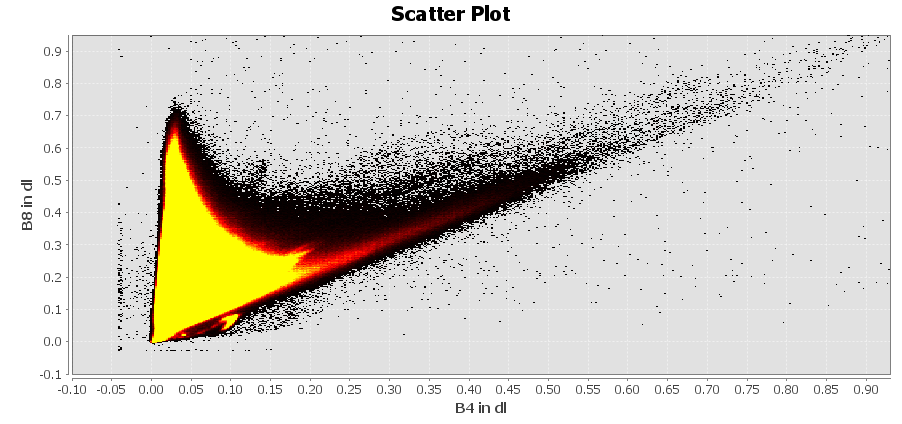
\includegraphics{./images/spectral_feature_space_vege_B04_B08.png}

}

\caption{\label{fig-vege}Spectral Feature Space, Vegetation On Bands B04
and B08}

\end{figure}

``Spectral Feature Space, Vegetation On Bands B04 and B08''

One of the applications really attracted me was the spatial signature of
vegetation on the terra, as we could assign features to each end of the
spatial signature area see Figure~\ref{fig-vege}, such as bare land on
the right end of the triangle-like area where red light captured are
dense while near-infrared level is low. Heavy vegetation are witnessed
at the upper end of the triangle-like area where red light low and
near-infrared is high, indicating heavy biomass. As for the left-down
corner where both red and near-infrared are low, we can identify wet
lands. This is integrated in the NDVI (Normalized Difference Vegetation
Index) to estimate vegetation cover.

\begin{figure}

{\centering 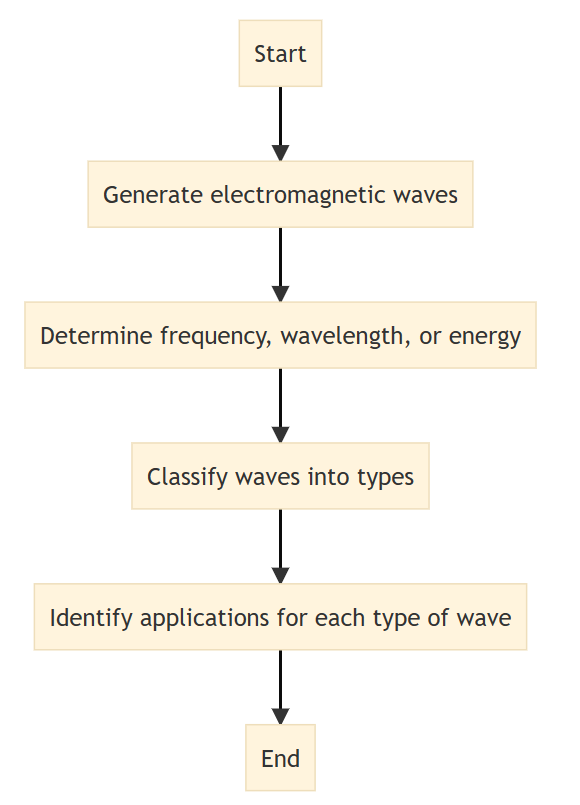
\includegraphics{./images/workflow of the Electromagnetic Spectrum.png}

}

\caption{\label{fig-wkfl}workflow of the Electromagnetic Spectrum}

\end{figure}

Spatial signatures can also be used to monitor the health of vegetation
by identifying patterns of quavariation in spectral reflectance that are
indicative of stress or disease. For example, vegetation that is
stressed or diseased may have a different spectral reflectance signature
than healthy vegetation, which can be identified using spatial
signatures.

In addition, spatial signatures can be used to monitor the growth and
distribution of vegetation over time by comparing satellite imagery from
different dates. This can be useful for understanding the impacts of
land use changes, climate change, and other factors on vegetation.

Overall, spatial signatures are a powerful tool for vegetation
monitoring, as they can be used to identify and classify different types
of vegetation, monitor vegetation health, and track vegetation changes
over time.

\hypertarget{reflection}{%
\section{Reflection}\label{reflection}}

Having active sensing methods is inspiring as it reminds us that instead
of struggling with improving image quality sensed passively using
sunlight, we can try altering to artificial signals. Also that sunlight
is but another form of electromagnetic wave. This implies a potential to
cancel the boundary between natural phenomenon and artificial forms. I
feel more encouraged to more actively explore relationships in nature
with the devices at hand. I am considering implement active sensors to
include SAR data for IoT-based data pipelines. With active sensing data
like SAR monitoring forestry real-time, the machine learning model can
acquire enough ground truth data from nature for constant adaptation.
This could be incorporated into forestry monitoring systems and disaster
monitoring systems to cover for both accuracy and rapidness.

One of the challenges I encountered is to navigate the complexities of
the interface of SNAP and QGIS. It becomes clear to me that yes
implementing several functions in code can be challenging, but a
software with collective functions as a whole can be mindblowing even
when with decent GUIs. Specifically, finding which function falling
under which menu consumes a lot of time, and figuring out filling
parameters to carry the analysis also took some efforts of iterative
validation. Anyway, it's nice to have attempts of designing GUIs for EO
data manipulation. Hopefully, with Large Language Model simplifying GIS
software designing, we can more easily translate code workflows into
user-friendly interfaces and apply our design ideas.

\bookmarksetup{startatroot}

\hypertarget{week-2---portfolio}{%
\chapter{Week 2 - Portfolio}\label{week-2---portfolio}}

\begin{itemize}
\tightlist
\item
  \href{https://andrewmaclachlan.github.io/CASA0023/2_portfolio.html}{Introducing
  Xaringan}
\end{itemize}

\bookmarksetup{startatroot}

\hypertarget{week-3---remote-sensing-data}{%
\chapter{Week 3 - Remote sensing
data}\label{week-3---remote-sensing-data}}

In this week's learning diary, we try to handle

\hypertarget{summary-1}{%
\section{Summary:}\label{summary-1}}

\hypertarget{different-sensors}{%
\subsection{Different Sensors}\label{different-sensors}}

Across track scanners: Mirror reflects light onto 1 detector. For
example, \uline{Landsat} dataset are captured by this sort

Along track scanners: Basically several detectors pushed along. E.g.,
Quickbird, SPOT

\hypertarget{geometric-correction}{%
\subsection{Geometric Correction}\label{geometric-correction}}

RS data could include image distortions introduced by: View angle,
topography, wind and rotation of the earth

We identify Ground Control Points (GCP) in distorted data to match them
with local map, correct image, or GPS data from handheld device, but
these reference images could also contain distortions and imprecisions.

RMSE is adopted here to measure fitness between images. Use GCPs to
minimise RMSE.

Doing geometric correction can shift the original image, so we want to
re-sample the final raster by using Nearest Neighbour, Linear, Cubic,
Cubic spline re-samplers

\hypertarget{atmosphric-correction}{%
\subsection{Atmosphric Correction}\label{atmosphric-correction}}

According to Jensen (1986), two factors contribute to environmental
attenuation: Atmospheric scattering, topographic attenuation.

There are unnecessary and necessary atmospheric corrections:

necessary ones are:

\begin{itemize}
\item
  Biophysical parameters needed (e.g.~temperature, leaf area index,
  NDVI)
\item
  E.g. .. .NDVI is used in the Africa Famine Early Warning System and
  Livestock Early Warning System
\item
  Using spectral signatures through time and space
\end{itemize}

Absorption and scattering can create the haze, i.e.~reduces contrast of
image.

Scattering can create the ``adjacency effect'', radiance from pixels
nearby mixed into pixel of interest.

\hypertarget{orthorectification-correction}{%
\subsection{Orthorectification
Correction}\label{orthorectification-correction}}

This is a subset of georectification, i.e.~giving coords to an image.
Particularly Orthorectification means removing distortion so pixels can
appear being viewed at \uline{nadir} (straight down). This requires the
support of an Elevation Model to calculate the nadir view for each pixel
on a sensor geometry.

To do this: cosine correction, Minnaert correction, Statistical
Empirical correction, C Correction (advancing the Cosine). Need radiance
(DN to TOA) from sloped terrain, Sun's zenith angle, Sun's incidence
angle - cosine of the angle between the solar zenith and the normal line
of the slope. Latter two found in angle coefficient files (e.g.~Landsat
data ANG.txt).

\hypertarget{rdiometric-correction}{%
\subsection{Rdiometric Correction}\label{rdiometric-correction}}

Corrections to raw satellite imagery can be performed using a method
called Dark Object Subtraction (DOS). The logic is that the darkest
pixel in the image should be 0 and any value it has is due to the
atmosphere. To remove the atmospheric effect, the value from the darkest
pixel is subtracted from the rest of the pixels in the image. The
calculation involves converting the Digital Number (DN) to radiance,
computing the haze value for each band (but not beyond NIR), and
subtracting the 1\% reflectance value from the radiance. The calculation
requires values such as mean exoatmospheric irradiance, solar azimuth,
Earth-sun distance, and others, which can be found in sources such as
Landsat user manuals.

\hypertarget{joining-data-sets}{%
\subsection{Joining data sets}\label{joining-data-sets}}

Also known as \uline{Mosaicking}: We feather two images, creating a
\uline{seamless} mosaic, where the diving lien is called
\uline{seamline}.

\hypertarget{image-enhancements}{%
\subsection{Image Enhancements}\label{image-enhancements}}

Image stretch, Band ratioing, Normalised Burn Ratio, Edge enhancement,
Filtering, PCA, Image fusion (see application) etc.

\hypertarget{application---discussing-image-fusion-in-one-literature}{%
\section{Application - Discussing image fusion in one
literature}\label{application---discussing-image-fusion-in-one-literature}}

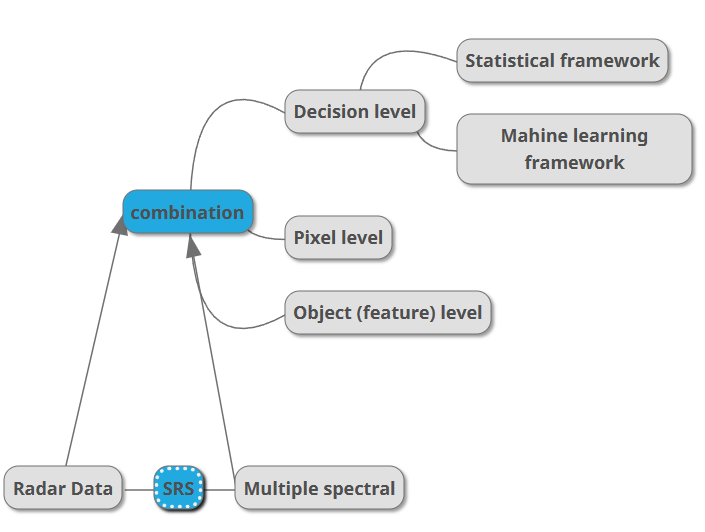
\includegraphics{./images/image-620878088.png}

From literature we delve in the nuances of levels on which we perform
image fusion to acquire better results. The integration methods vary as
the levels vary (Schulte to Bühne and Pettorelli 2018).

Satellite remote sensing (SRS) can be derived from Multispectral sensors
and radar sensors.~

~Multispectral sensors are passive, merely receiving electromagnetic
waves reflected from surface, usually used to reflect chemical
properties (such as nitrogen or carbon content and moisture). Usually
produces data with comparatively low spatial resolution

~Radar ones emit electromagnetic radiation and measure the returning
signal, responding to the three-dimensional structure of objects, being
sensitive to their orientation, volume and surface roughness. Usually
produces data with comparatively high spatial resolution

\hypertarget{image-fusion}{%
\subsection{Image fusion:}\label{image-fusion}}

1.~\textbf{decision-level}~(SRS integration), where separate predictors
are used to estimate a parameter of interest.~

2.~\textbf{object-level (feature-level).}~unit: multi-pixel objects. (1)
using radar and multispectral imagery is input into an object-based
image segmentation algorithm, or (2) segmenting each type of imagery
separately before combining them. multi-pixel objects

3.~\textbf{pixel-level (Observation-level)}, where pixel values are
combined to derive a fused image with new pixel values, either in the
spatial or the temporal domain.

(2. and 3. derive entirely new predictors.)

\begin{figure}

{\centering 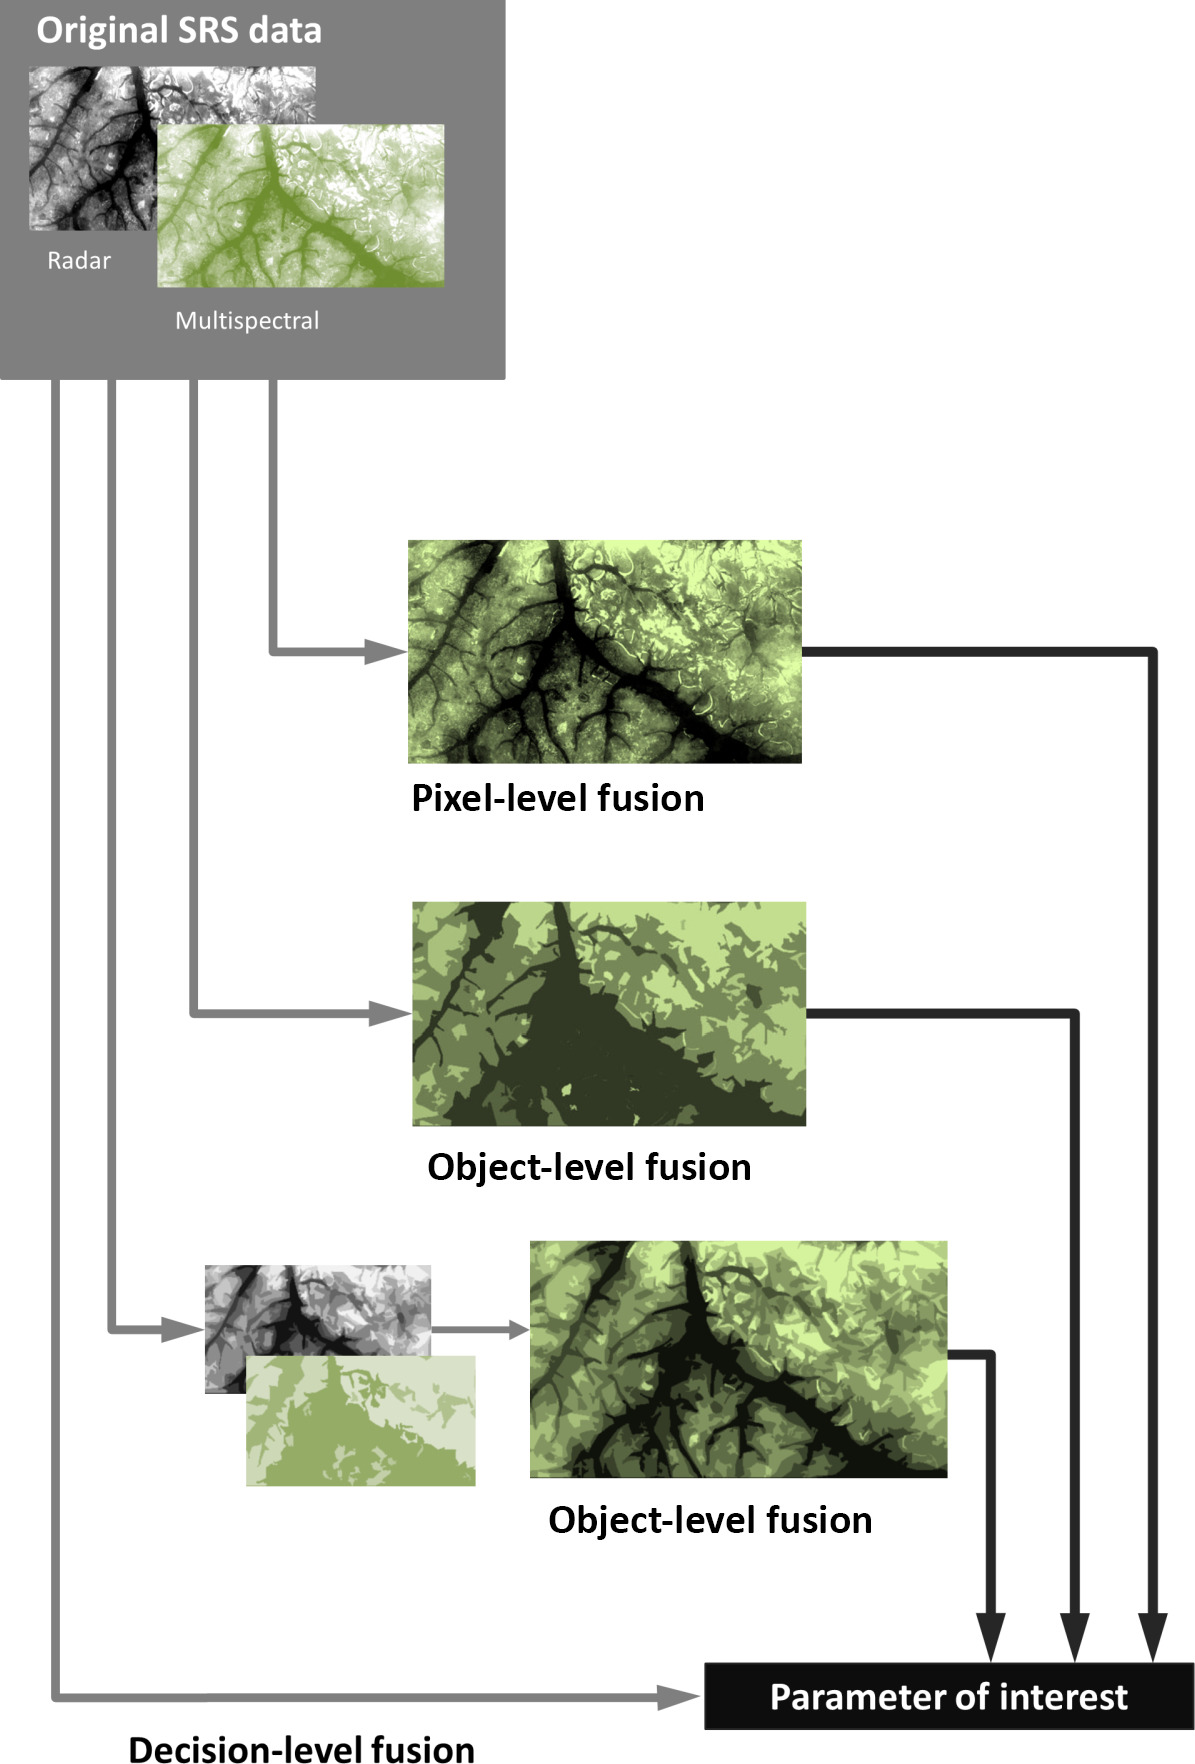
\includegraphics{./images/fusion techniques.png}

}

\caption{\label{fig-fusiontech}Credit: Schulte to Bühne and Pettorelli
(2018)}

\end{figure}

Schematic overview of multispectral-radar SRS data fusion techniques.
The parameter of interest can be a categorical variable, like land
cover, or a continuous variable, like species richness. In pixel-level
fusion, the original pixel values of radar and multispectral imagery are
combined to yield new, derived pixel values. Object-based fusion refers
to (1) using radar and multispectral imagery is input into an
object-based image segmentation algorithm, or (2) segmenting each type
of imagery separately before combining them. Finally, decision-level
fusion corresponds to the process of quantitatively combining
multispectral and radar imagery to derive the parameter of interest (by
e.g.~combining them in a regression model, or classification algorithm)

\hypertarget{implementation-approaches}{%
\subsection{Implementation Approaches}\label{implementation-approaches}}

\begin{figure}

{\centering 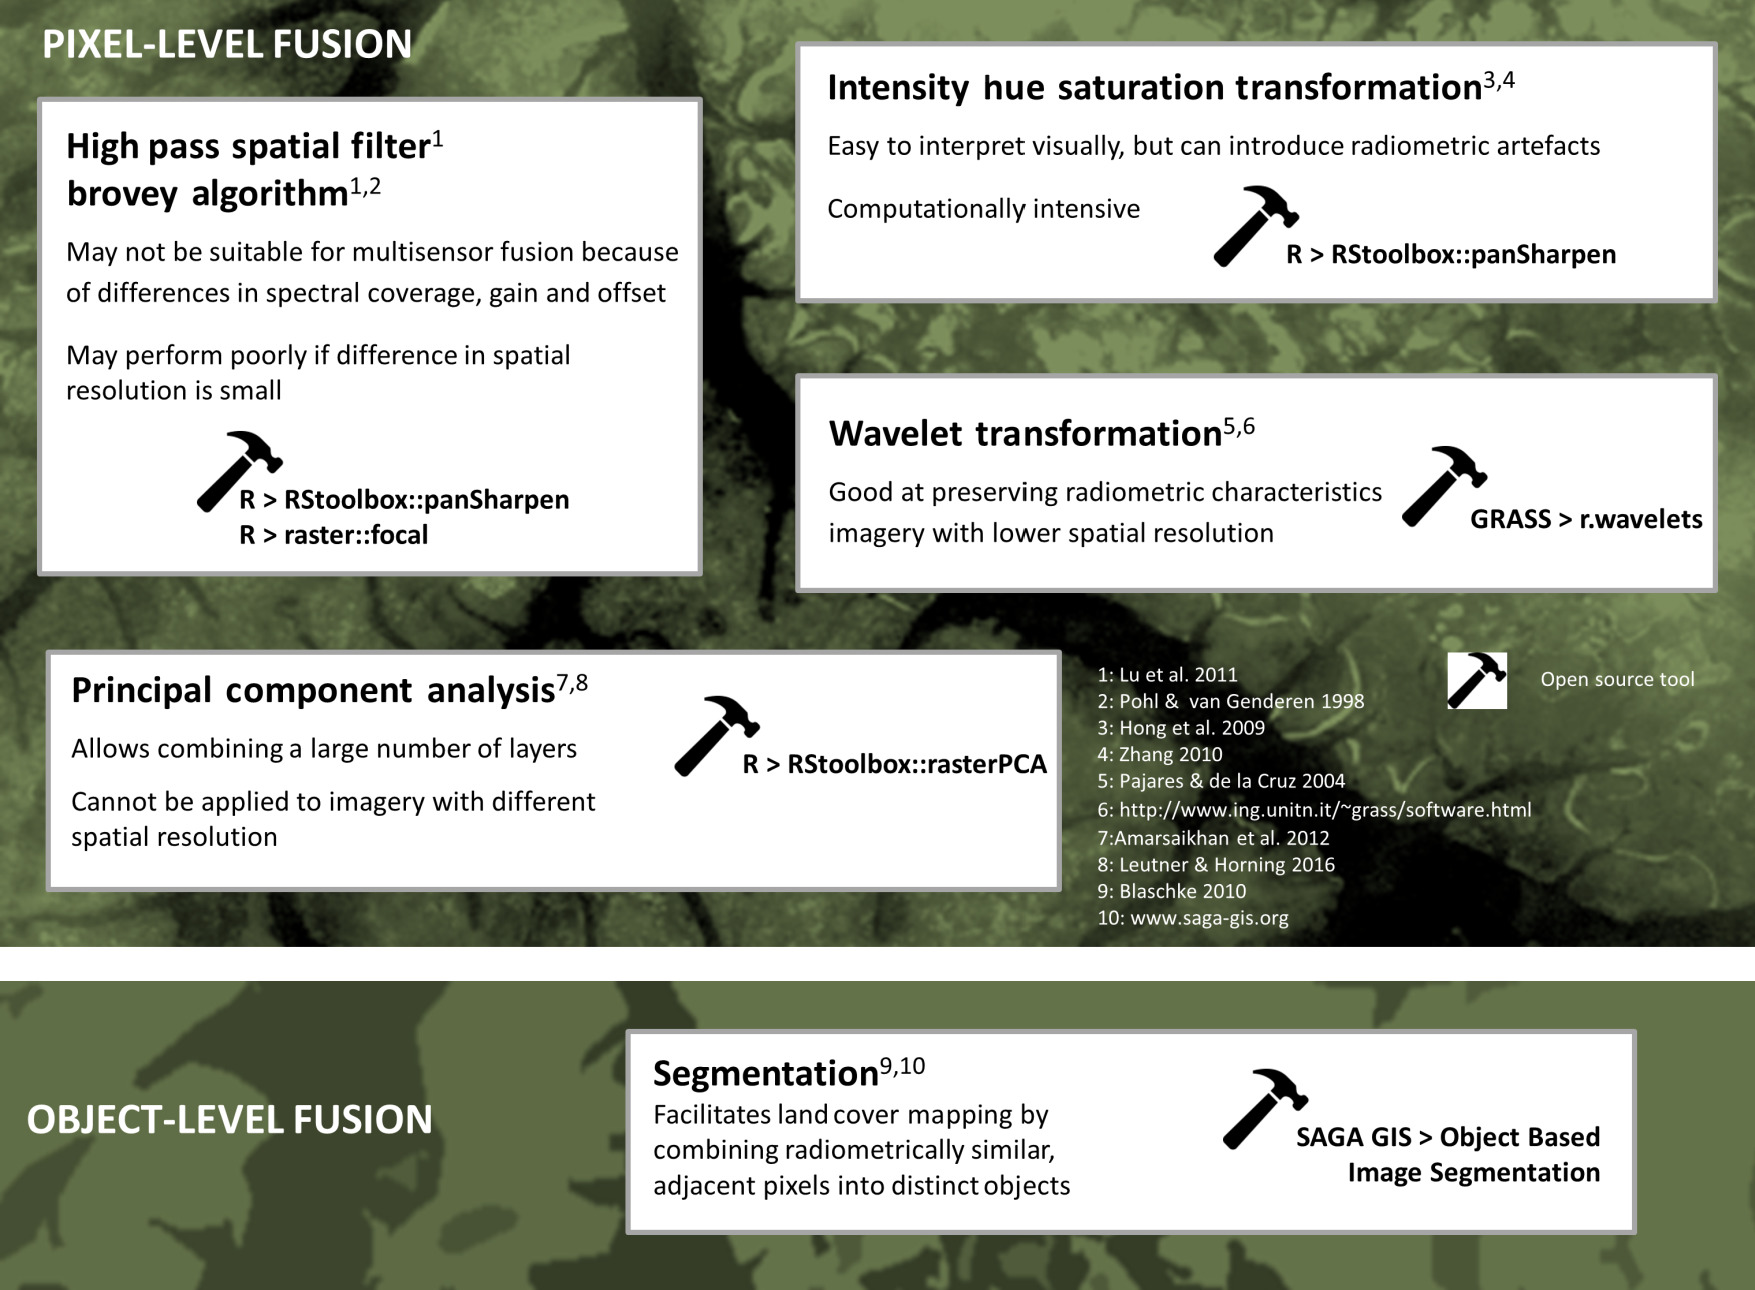
\includegraphics{./images/Implementation approach.png}

}

\caption{\label{fig-impleApproach}Credit: Schulte to Bühne and
Pettorelli (2018)}

\end{figure}

\textbf{\emph{pixel-level}}

\begin{enumerate}
\def\labelenumi{\arabic{enumi}.}
\tightlist
\item
  Component substitution techniques: such as principal component
  analysis (PCA), Intensity-hue-saturation (IHS).~\\
\item
  PCA is the only pixel-level image fusion technique that cannot be
  applied to imagery with different spatial resolutions, and the only
  that allows unlimited image numbers.\\
\item
  IHS fusion. Three images with lower spatial resolution (typically
  multispectral data) are integrated with a single image with high
  spatial resolution (typically radar) to retain the radiometry but
  increase the spatial resolution of the former. Facilitate visual
  interpretation by combining resulting images into a single RGB
  image.\\
\item
  Multi-resolution analysis,~such as~**Wavelet transformation. Decompose
  multispectral and radar imagery into their respective low- and
  high-frequency components\\
\item
  Arithmetic fusion techniques:~such as the Brovey transform algorithm.
  Unlikely to be appropriate for multispectral-radar SRS image fusion.
\end{enumerate}

\textbf{\emph{Object-level}}:~Based on brightness and intensity values
of each pixel, as well as its spatial context, objects such as lines,
shapes or textures are extracted.

1.~\textbf{image segmentation:} Demands that multispectral and radar SRS
images are with the same spatial resolution

2.~*extracting objects separately and combining in a feature map*

Object-based fusion reduces all multispectral and radar information into
a single layer of discrete objects, which are often relatively easy to
relate to ecological features.

\textbf{\emph{Decision-level fusion}}: Quantitative decision-making
frameworks---such as a regression, a quantitative model or a
classification algorithm.

\hypertarget{reflection-1}{%
\section{Reflection}\label{reflection-1}}

Data correction, Data fusion and Image enhancement SRS data fusion can
increase the quality of SRS (Satellite Remote sensing)-derived
parameters for application in terrain detection, urban analysis, ecology
and conservation (Schulte to Bühne and Pettorelli 2018). It is thus
important to explore how best to capitalise on recent technological
developments and changes in SRS data availability. It is exctiing to
apply solid machine learning methods to this area and it is marvelous to
see the progress reflected by the increasing number of software
supporting this application. The improvement of image quality enables
new research designs in ecology and conservation areas and reignite
previously greyed-out options.

The application of data correction, data fusion, and image enhancement
techniques to SRS data can greatly improve the accuracy and reliability
of SRS-derived parameters, which can then be used in various fields,
including terrain detection, urban analysis, ecology, and conservation.
With the rapid advancements in technology and the increasing
availability of SRS data, there is a growing opportunity to leverage the
latest machine learning techniques in this area. The development of new
software tools to support these applications is a testament to the
progress being made in this field. By enhancing the quality of the SRS
data, researchers are able to design more robust and informative
studies, unlocking new insights and avenues for exploration in ecology
and conservation. This, in turn, has the potential to lead to
breakthroughs and innovations in these fields, making a significant
impact on the world around us.

\bookmarksetup{startatroot}

\hypertarget{week4---policy-case-study-in}{%
\chapter{Week4 - Policy Case Study
in}\label{week4---policy-case-study-in}}

\href{https://onenyc.cityofnewyork.us/wp-content/uploads/2019/05/OneNYC-2050-Summary.pdf}{OneNYC-2050-Summary.pdf
(cityofnewyork.us)}

\hypertarget{summary-2}{%
\section{Summary}\label{summary-2}}

\hypertarget{application-1}{%
\section{Application}\label{application-1}}

The initiatives provided cover a wide range of areas, including
education, small business support, community resilience, infrastructure,
transportation, and sustainability. One of the key applications of these
initiatives is to improve the quality of life for New Yorkers,
particularly those in underrepresented communities. For example, the
initiatives aimed at increasing the number of New Yorkers earning a high
school equivalency diploma and connecting underrepresented groups to
construction jobs created by City investments are designed to provide
greater economic opportunities and upward mobility.

Similarly, the initiatives aimed at enhancing walkability and
accessibility and improving the sustainability and efficiency of air
travel are designed to improve the physical infrastructure of the city
and make it more accessible and sustainable for all residents. Another
application of these initiatives is to promote equity and inclusivity in
the city.

Many of the initiatives are specifically targeted at underrepresented
communities, such as the initiatives aimed at providing paid internships
and professional development opportunities to cultural workers and
supporting the growth and retention of small businesses.

By providing resources and support to these communities, the city aims
to promote greater equity and inclusivity and reduce disparities in
access to resources and opportunities.

The initiatives also reflect a commitment to sustainability and
resilience. Many of the initiatives are aimed at improving the city's
infrastructure and transportation systems to make them more sustainable
and resilient in the face of climate change and other challenges. For
example, the initiatives aimed at investing in innovative and resilient
transportation networks and enhancing walkability and accessibility are
designed to reduce emissions and congestion and promote sustainable
modes of transportation.

Overall, the initiatives outlined in the text reflect a comprehensive
and multi-faceted approach to improving life in New York City. While
there is still much work to be done, these initiatives represent an
important step forward in promoting equity, sustainability, and
resilience in the city. As future literature advancements are made, it
will be important to continue to evaluate and refine these approaches to
ensure that they are effective and responsive to the needs of all New
Yorkers.

\hypertarget{reflection-2}{%
\section{Reflection}\label{reflection-2}}

The initiatives outlined in the text cover critical components of urban
planning and development, including infrastructure, transportation,
education, and sustainability. The initiatives outlined in the text
emphasize the importance of investing in the city's data infrastructure
and establishing a citywide data catalog, among other things. This
requires a deep understanding of data management and analysis
techniques, as well as the ability to work with large and complex
datasets. Spatial data scientists and deep learning solution engineers
can use these skills to develop innovative solutions for urban planning
and development, such as predictive models for traffic flow or energy
consumption.

Many of the initiatives outlined in the text involve the use of GIS
products and services, as well as the expansion of walkability and
accessibility in the city. This requires a deep understanding of
geospatial data analysis techniques, as well as the ability to work with
mapping and visualization tools. Spatial data scientists and deep
learning solution engineers can use these skills to develop innovative
solutions for urban planning and development, such as interactive maps
that show the most walkable routes in the city.

In addition to these skills, the content, data, and tools presented in
the text are highly relevant to the broader discipline of urban planning
and development. Spatial data scientists and deep learning solution
engineers can use these resources to develop innovative solutions for a
wide range of urban challenges, from improving transportation networks
to promoting sustainability and resilience. By leveraging these
resources, these professionals can help to create more livable and
equitable cities that meet the needs of all residents. Looking to the
future, it will be important for spatial data scientists and deep
learning solution engineers to continue to stay up-to-date with the
latest advancements in data management, analysis, and visualization
techniques.

\bookmarksetup{startatroot}

\hypertarget{week-5---an-introduction-to-google-earth-engine}{%
\chapter{Week 5 - An introduction to Google Earth
Engine}\label{week-5---an-introduction-to-google-earth-engine}}

This week introduces \textbf{Google Earth Engine (GEE)}, a geospatial
processing service that allows for planetary scale analysis of massive
datasets in seconds.

Basics:

\begin{itemize}
\tightlist
\item
  The set up of GEE, its terms and jargon, and client vs server side
  operations, see Table 1
\item
  How GEE uses Javascript and how mapping functions are used instead of
  loops
\item
  The concept of scale in GEE, which refers to both the volume of
  analysis and pixel resolution
\item
  How GEE aggregates the image to fit a 256x256 grid.
\end{itemize}

Objects and methods in GEE are introduced:

\begin{itemize}
\tightlist
\item
  E.g. geometries, features, feature collections, and
\item
  Various data reduction techniques (e.g., reducing images, reducing
  images by region(s), reducing images by neighborhood).
\end{itemize}

Also, the types of analyses that can be performed in GEE are briefly
covered.

\hypertarget{summary-3}{%
\section{Summary}\label{summary-3}}

Introduced GEE Basics, Objects, Geometries and applications.

Table 1: Terms, Jargon, and Processes Related to Google Earth Engine

\begin{longtable}[]{@{}
  >{\raggedright\arraybackslash}p{(\columnwidth - 4\tabcolsep) * \real{0.0761}}
  >{\raggedright\arraybackslash}p{(\columnwidth - 4\tabcolsep) * \real{0.1117}}
  >{\raggedright\arraybackslash}p{(\columnwidth - 4\tabcolsep) * \real{0.8122}}@{}}
\toprule()
\begin{minipage}[b]{\linewidth}\raggedright
Category
\end{minipage} & \begin{minipage}[b]{\linewidth}\raggedright
Term/Aspect
\end{minipage} & \begin{minipage}[b]{\linewidth}\raggedright
Definition
\end{minipage} \\
\midrule()
\endhead
Basics & Google Earth Engine & A geospatial processing service that
allows geospatial analysis at scale. \\
Basics & Image & Refers to raster data in GEE and has bands. \\
Basics & Feature & Refers to vector data in GEE and has geometry and
attributes. \\
Basics & ImageCollection & A stack of images in GEE. \\
Basics & FeatureCollection & A stack of features (lots of polygons) in
GEE. \\
Basics & Proxy objects & GEE objects that are stored on the server and
have no data in the script. \\
Objects & Earth Engine Objects & Objects in GEE starting with ``ee''. \\
Objects & Images (Rasters) & GEE object representing raster data with
bands. \\
Objects & Feature & GEE object representing vector data with geometry
and attributes. \\
Objects & ImageCollection & A stack of images in GEE. \\
Objects & FeatureCollection & A stack of features (lots of polygons) in
GEE. \\
Objects & Joins & Combining two FeatureCollections with a common
property. \\
Objects & Arrays & Used to store and manipulate lists of values. \\
Objects & Chart & Used to visualize data in GEE. \\
Geometry & Point & A single location represented by its longitude and
latitude. \\
Geometry & Line & A series of connected points representing a linear
feature. \\
Geometry & Polygon & A closed shape with three or more sides,
represented by a series of connected lines forming a closed loop. \\
Geometry & MultiPolygon & A collection of polygons, where each polygon
is represented as a list of coordinate tuples defining its vertices. \\
Geometry & MultiGeometry & A collection of different types of
geometries. \\
Processes & Reducing & Summarizing data over a specified dimension or
property. \\
Processes & Filtering & Reducing data to a specific subset based on a
specified condition. \\
Processes & Mapping & Applying a function to every element of a
collection in GEE. \\
Processes & Scaling & Refers to the pixel resolution in GEE. The scale
is set by the output, not the input, and Earth Engine selects the
pyramid with the closest scale to analysis. \\
Client/Server & Client Side & Refers to the browser side of GEE. \\
Client/Server & Server Side & Refers to the side of GEE where data is
stored. \\
Client/Server & Looping & Looping is not recommended for objects on the
server side. \\
Client/Server & Mapping & Instead of loops, mapping is used in GEE to
apply a function to everything on the server. \\
\bottomrule()
\end{longtable}

\hypertarget{gee-basics}{%
\subsection{GEE Basics}\label{gee-basics}}

JavaScript, where objects are dictionaries:

\begin{itemize}
\tightlist
\item
  We have ee (EarthEngine), a powerful package. Anything starting with
  ee (proxy objects) are stored on the server.
\item
  Problems:

  \begin{itemize}
  \tightlist
  \item
    We don't iterate the data on the server; instead, we map (using a
    mapping function) them into objects (variables) so we only load them
    once.
  \item
    There are also some sort of server-wide functions.
  \item
    Avoid using loops in GEE on the server-side, as mapping can
    automatically detect the number of loops needed.
  \end{itemize}
\end{itemize}

Scale:

\begin{itemize}
\tightlist
\item
  Pixel resolution, set by the output.
\item
  GEE does resampling, aggregating your input to a 256*256, mainly
  down-sampling.
\end{itemize}

\hypertarget{gee-objects}{%
\subsection{GEE Objects}\label{gee-objects}}

Objects:

\begin{itemize}
\tightlist
\item
  Images (Rasters), geometry, ImageCol, features, featureCol, joins,
  arrays, chart.
\end{itemize}

\hypertarget{gee-processes-and-applicationsoutputs}{%
\subsection{GEE Processes and
Applications/Outputs}\label{gee-processes-and-applicationsoutputs}}

GEE applications:

\begin{itemize}
\tightlist
\item
  Reducing types.
\item
  Different to filterBounds() that filters the area of interest, to do
  zonal statistics, we have reduceRegion(), where regions are
  subcategories of the area of interest.
\item
  Also, we have reduceNeighborhood(), which is a bit like a kind of
  image enhancement.
\end{itemize}

Linear Regressions:

\begin{itemize}
\tightlist
\item
  In a scenario of visualising precipitation, we can do a multivariate
  multiple linear regression where both independent variables (time) and
  dependent (precip, temp) variables are multiple.
\item
  Something about constant bound.
\end{itemize}

Joins:

\begin{itemize}
\tightlist
\item
  In GEE, everything, e.g.~within a buffer, intersect, etc. needs the
  mediation of Join (apply()).
\item
  To perform joins, we need to put data into Filter().
\end{itemize}

Classifiers:

\begin{itemize}
\tightlist
\item
  Per-pixel
\item
  sub-pixel
\end{itemize}

Table 2: GEE Processes and Applications/Outputs

\begin{longtable}[]{@{}
  >{\raggedright\arraybackslash}p{(\columnwidth - 2\tabcolsep) * \real{0.1265}}
  >{\raggedright\arraybackslash}p{(\columnwidth - 2\tabcolsep) * \real{0.8735}}@{}}
\toprule()
\begin{minipage}[b]{\linewidth}\raggedright
Process
\end{minipage} & \begin{minipage}[b]{\linewidth}\raggedright
Description
\end{minipage} \\
\midrule()
\endhead
Geometry operations & Spatial operations such as union, intersection,
buffer, and distance analysis \\
Joins & Combining two feature collections based on a shared attribute
value \\
Zonal statistics & Computing statistics for a region or set of regions
such as mean, median, and mode of pixel values within a feature or a
collection of features \\
Filtering & Filtering of images or specific values based on criteria
such as date range, location, and attribute value \\
Machine learning & Using statistical and machine learning algorithms for
classification, clustering, and prediction tasks \\
Deep learning & A subset of machine, using Deep Neural Networks \\
\bottomrule()
\end{longtable}

\hypertarget{advantages-and-limitations}{%
\subsection{Advantages and
Limitations}\label{advantages-and-limitations}}

\begin{longtable}[]{@{}
  >{\raggedright\arraybackslash}p{(\columnwidth - 2\tabcolsep) * \real{0.4842}}
  >{\raggedright\arraybackslash}p{(\columnwidth - 2\tabcolsep) * \real{0.5158}}@{}}
\toprule()
\begin{minipage}[b]{\linewidth}\raggedright
Pros
\end{minipage} & \begin{minipage}[b]{\linewidth}\raggedright
Cons
\end{minipage} \\
\midrule()
\endhead
1. Large-scale data processing & 1. Limited to Google's data catalog \\
2. Access to vast satellite imagery library & 2. Steeper learning curve
for beginners \\
3. Real-time data analysis capabilities & 3. Requires coding skills
(JavaScript, Python) \\
4. Cloud-based platform & 4. Limited customization options \\
5. Free for non-commercial use & 5. Data export restrictions \\
6. Easy data sharing and collaboration & 6. Dependent on internet
connectivity \\
\bottomrule()
\end{longtable}

*No support for phase data, needs SNAP.

\hypertarget{trend}{%
\subsection{Trend}\label{trend}}

See also Section Application for details and references.

\begin{enumerate}
\def\labelenumi{\arabic{enumi}.}
\tightlist
\item
  Enhancement user interface: GEE might introduce a more user-friendly
  interface to lower the entry barrier for beginners and
  non-programmers, making it more accessible to a wider audience.
\item
  Integration with machine learning and AI: GEE could expand its
  integration with advanced machine learning and AI algorithms, enabling
  users to derive more sophisticated insights from geospatial data.
\item
  Customisable solutions: GEE may introduce more customization options
  for users, allowing them to develop tailored geospatial analysis tools
  and applications.
\item
  Better support for commercial use: GEE could offer more comprehensive
  support and licensing options for commercial users, helping businesses
  harness the full potential of geospatial data analysis.
\end{enumerate}

\hypertarget{application-2}{%
\section{Application}\label{application-2}}

Literature choice: Gorelick et al. (2017).

This week's recommended literature mainly are documentation support for
GEE and literature, even papers. Therefore the contribution of the
literature will be in more general senses. An overview of Google Earth
Engine's capabilities and applications, as well as its potential to
address societal issues.

They also discuss potential future developments, including expanding
Earth Engine's data catalog, improving its user interface, and
increasing collaboration with other organizations.

\begin{itemize}
\tightlist
\item
  Expanding Earth Engine's data catalog: currently includes a wide range
  of geospatial datasets but could be expanded to include additional
  sources of data (Gorelick et al. 2017).
\item
  Improving the user interface: make it more intuitive and
  user-friendly, particularly for non-expert users.
\item
  Increasing collaboration with other organizations: Collaboration with
  other organizations, both in terms of data sharing and joint research
  projects, is also an important area for future development.
\item
  Ongoing research into new analysis techniques and algorithms: Ongoing
  research into new analysis techniques and algorithms will continue to
  expand Earth Engine's capabilities and applications (Moore and Hansen
  2011).
\end{itemize}

\hypertarget{reflection-3}{%
\section{Reflection}\label{reflection-3}}

GEE-using skills can be a valuable asset for a spatial data scientist,
as it allows for complex spatial analysis at scale. Traditional GIS
software are eclipsed when it comes to both efficiency and scale.

GEE's unique and efficient way of conducting analysis flows is
interesting, such as the introduction of concepts like client vs
server-side operations and data reduction techniques. These was required
by GEE's feature of carrying out analyses on massive datasets (Gorelick
et al. 2017). For those interested in BigData technology, the strategies
(server/client split, no looping on server, etc.) applied by Google here
is a very resourceful one and worth learning. The user end also has to
learn to adopt good practices for reducing data range, which has been
simplified to a series of reduction and filtering functions,
e.g.~\texttt{ImageCollection.filterDate(),\ image.reduceNeighborhood()}(Google
2023b).

GEE's combination with machine learning is also promising in regard of
automating complex analysis tasks, as Machine Learning APIs offered by
GEE support Supervised and Unsupervised Classification, and Regression
(Google 2023a). According to Saad El Imanni et al. (2023), as a subtask
of intelligent agriculture, weeds detection task sees an impressive
performance (overall accuracy reached 96.87\%) when GEE and Machine
learning are combined.

In conclusion, I believe familiarity with GEE will add to one's machine
learning workflow in dealing with EO data, and, more generally,
incredibly large datasets. The design of GEE also opens an era of
web-service based big-data handling. Its designs in alleviating
computation on client side and getting rid of for-loop on server-side
inspires service designers to make distinct standards for code practice
based on the server-client split. Besides, the sheer amount and diverse
categories of data available on GEE saves experts from burdensome data
collection process, so they can focus more on EO data processing,
analysis and storytelling.

\bookmarksetup{startatroot}

\hypertarget{wk6-classification}{%
\chapter{Wk6 Classification}\label{wk6-classification}}

\hypertarget{summary-4}{%
\section{Summary}\label{summary-4}}

\begin{longtable}[]{@{}
  >{\raggedright\arraybackslash}p{(\columnwidth - 2\tabcolsep) * \real{0.2639}}
  >{\raggedright\arraybackslash}p{(\columnwidth - 2\tabcolsep) * \real{0.7361}}@{}}
\toprule()
\begin{minipage}[b]{\linewidth}\raggedright
Information
\end{minipage} & \begin{minipage}[b]{\linewidth}\raggedright
Summary
\end{minipage} \\
\midrule()
\endhead
Purpose of classification & To subset data into classes or values, such
as landcover or estimating values like GCSE scores or pollution. \\
Different classification methods & Essentially slice the data in
different ways. \\
Complexity of classification methods & They can often be made to appear
more complicated than they are. \\
Controlling classifiers & Can be done using hyperparameters. \\
Desired outcome of classifiers & Can range from a single tree to a
decision hyperplane boundary in multiple dimensions. \\
\bottomrule()
\end{longtable}

\hypertarget{ml-methods-in-eo-data-classification}{%
\subsection{ML methods in EO data
classification}\label{ml-methods-in-eo-data-classification}}

Table 1: Supervised Classification Methods

\begin{longtable}[]{@{}
  >{\raggedright\arraybackslash}p{(\columnwidth - 2\tabcolsep) * \real{0.2500}}
  >{\raggedright\arraybackslash}p{(\columnwidth - 2\tabcolsep) * \real{0.7500}}@{}}
\toprule()
\begin{minipage}[b]{\linewidth}\raggedright
Method
\end{minipage} & \begin{minipage}[b]{\linewidth}\raggedright
Description
\end{minipage} \\
\midrule()
\endhead
Maximum Likelihood & A statistical method used to estimate the
parameters of a probability distribution based on observed data. \\
Support Vector Machines (SVM) & A supervised learning algorithm that
finds the best hyperplane to separate data into different classes. \\
\bottomrule()
\end{longtable}

Table 2: Unsupervised Classification Methods

\begin{longtable}[]{@{}
  >{\raggedright\arraybackslash}p{(\columnwidth - 2\tabcolsep) * \real{0.2361}}
  >{\raggedright\arraybackslash}p{(\columnwidth - 2\tabcolsep) * \real{0.7639}}@{}}
\toprule()
\begin{minipage}[b]{\linewidth}\raggedright
Method
\end{minipage} & \begin{minipage}[b]{\linewidth}\raggedright
Description
\end{minipage} \\
\midrule()
\endhead
Density Slicing & Divides the range of pixel values into equal intervals
and assigns each interval a unique class value. \\
Parallelpiped & Uses a set of user-defined ranges for each band to
define class boundaries in multi-dimensional space. \\
Minimum Distance to Mean & Assigns each pixel to the class with the
closest mean value in multi-dimensional space. \\
Nearest Neighbor & Assigns each pixel to the class of its nearest
neighbor in multi-dimensional space. \\
\bottomrule()
\end{longtable}

Table 3: Other Machine Learning Methods

\begin{longtable}[]{@{}
  >{\raggedright\arraybackslash}p{(\columnwidth - 2\tabcolsep) * \real{0.2361}}
  >{\raggedright\arraybackslash}p{(\columnwidth - 2\tabcolsep) * \real{0.7639}}@{}}
\toprule()
\begin{minipage}[b]{\linewidth}\raggedright
Method
\end{minipage} & \begin{minipage}[b]{\linewidth}\raggedright
Description
\end{minipage} \\
\midrule()
\endhead
Artificial Neural Networks (ANN) & A set of algorithms inspired by the
structure and function of biological neural networks, used for pattern
recognition and prediction tasks. \\
\bottomrule()
\end{longtable}

\hypertarget{pros-and-cons---supervised-vs.-unsupervised}{%
\subsection{Pros and cons - Supervised
vs.~Unsupervised}\label{pros-and-cons---supervised-vs.-unsupervised}}

Table 1: Supervised vs.~Unsupervised Classification

\begin{longtable}[]{@{}
  >{\raggedright\arraybackslash}p{(\columnwidth - 4\tabcolsep) * \real{0.1918}}
  >{\raggedright\arraybackslash}p{(\columnwidth - 4\tabcolsep) * \real{0.5479}}
  >{\raggedright\arraybackslash}p{(\columnwidth - 4\tabcolsep) * \real{0.2603}}@{}}
\toprule()
\begin{minipage}[b]{\linewidth}\raggedright
Classification Type
\end{minipage} & \begin{minipage}[b]{\linewidth}\raggedright
Definition
\end{minipage} & \begin{minipage}[b]{\linewidth}\raggedright
Method
\end{minipage} \\
\midrule()
\endhead
Supervised & Classifier learns patterns in the data and uses that to
place labels onto new data. Pattern vector is used to classify the
image. Usually, pixels are treated in isolation but as we have seen -
contextual (neighboring pixels), objects (polygons), texture. & Pattern
recognition or machine learning \\
Unsupervised & Identifies land cover classes that aren't known a priori
(before) and tells the computer to cluster based on info it has
(e.g.~bands) and label the clusters. & Density slicing, parallelpiped,
minimum distance to mean, nearest neighbor, neural networks, machine
learning / expert systems* \\
\bottomrule()
\end{longtable}

\hypertarget{overfitting}{%
\subsection{Overfitting}\label{overfitting}}

\begin{itemize}
\tightlist
\item
  Bias refers to the difference between the predicted value and the true
  value. When a model has high bias, it is too simple and may underfit
  the data. On the other hand, when a model has low bias, it may overfit
  the data.
\item
  Variance, on the other hand, refers to the variability of a model for
  a given point. When a model has high variance, it is too complex and
  may overfit the data. This means that it will perform well on the
  training data but poorly on new data.
\end{itemize}

\begin{figure}

{\centering 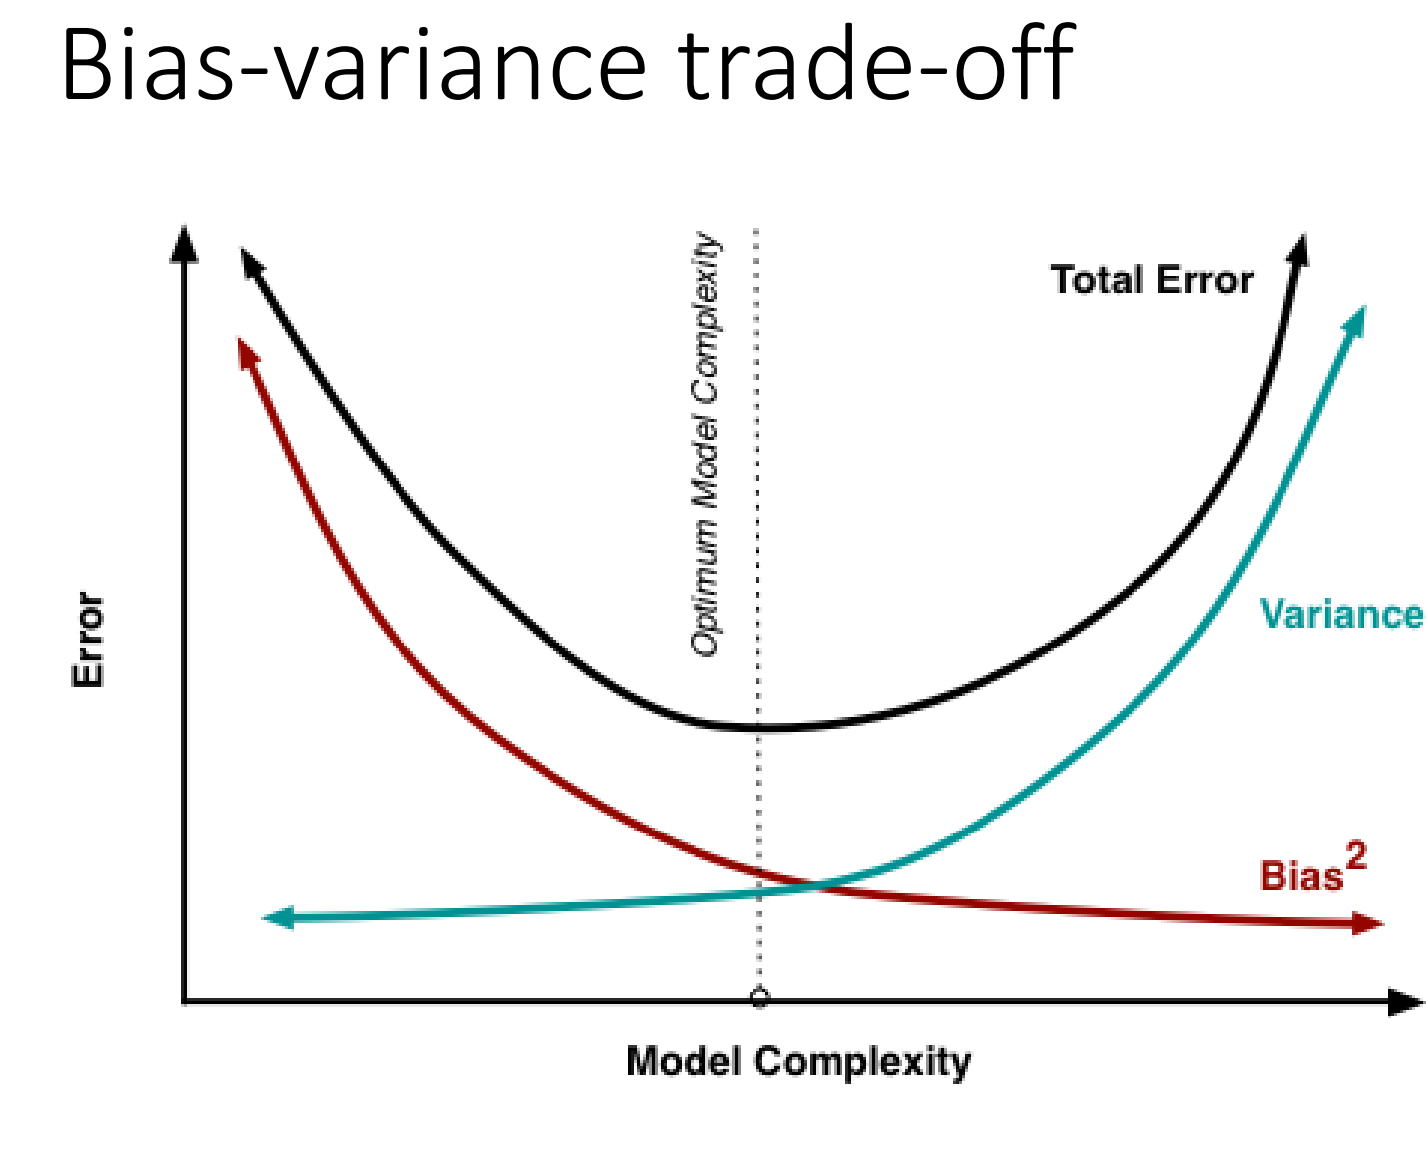
\includegraphics{./images/Bias-variance-01.png}

}

\caption{\label{fig-BiasVar01}Credit: CASA0006}

\end{figure}

In general, overfitting occurs when there is a trade-off between bias
and variance. A model with high bias and low variance will underfit the
data, while a model with low bias and high variance will overfit the
data. The goal is to find a balance between bias and variance that
results in good performance on both training and test data.

\begin{figure}

{\centering 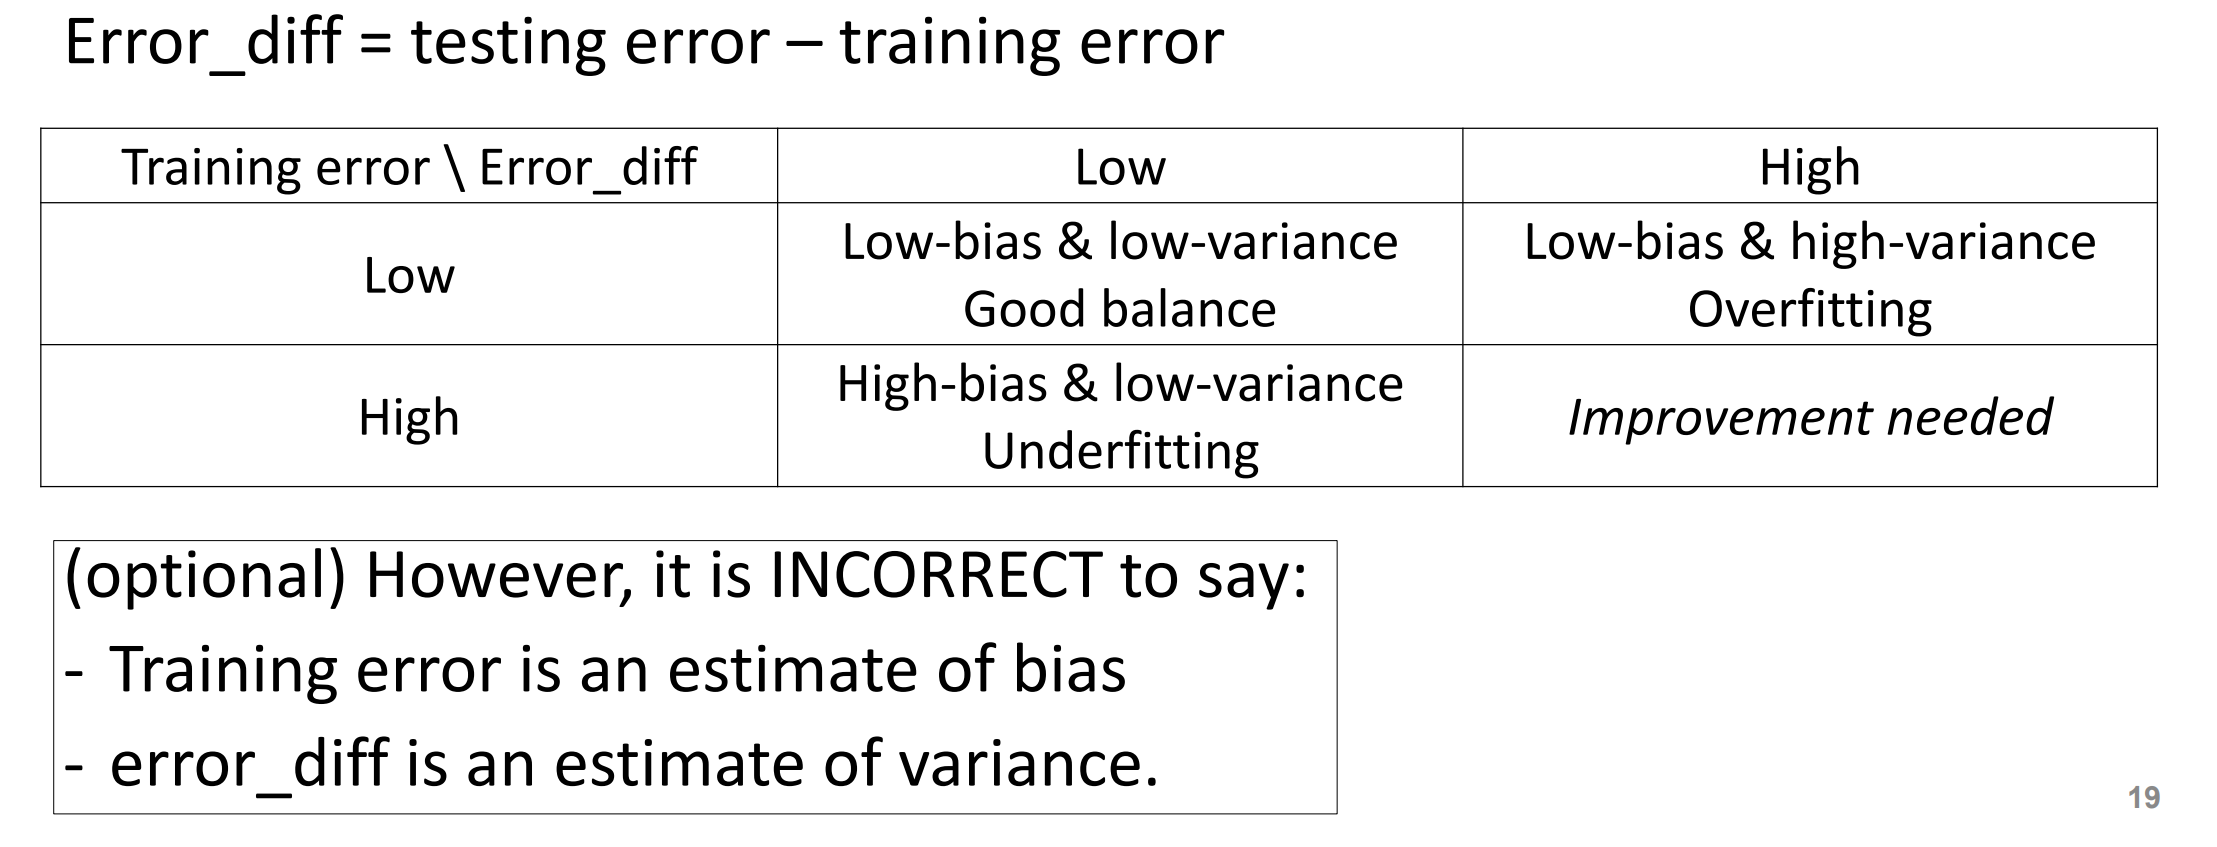
\includegraphics{./images/Bias-variance-02.png}

}

\caption{\label{fig-BiasVar02}Credit: CASA0006}

\end{figure}

\hypertarget{outlook-on-the-development-of-eo-data-classification}{%
\subsection{Outlook on the development of EO data
Classification}\label{outlook-on-the-development-of-eo-data-classification}}

Earth Observation (EO) data classification is continually evolving, with
new technologies and techniques leading to several anticipated future
developments:

\begin{enumerate}
\def\labelenumi{\arabic{enumi}.}
\tightlist
\item
  Multi-source data fusion:

  \begin{itemize}
  \tightlist
  \item
    Integrating data from multiple sources like satellite imagery,
    LiDAR, and ground-based sensors will become more prevalent. This
    fusion enhances classification accuracy and offers comprehensive
    Earth's surface information, improving decision-making and
    monitoring. For example, the European Union's
    \href{https://www.copernicus.eu/en}{\textbf{Copernicus Programme}}
    could use this in providing free data from various satellite
    missions and sensors for environmental monitoring, disaster
    management, and urban planning.
  \end{itemize}
\item
  Multi-temporal analysis:

  \begin{itemize}
  \tightlist
  \item
    Sophisticated multi-temporal analysis techniques will be
    increasingly used to monitor changes in land cover, vegetation, and
    other features over time. This enables accurate and efficient change
    detection and monitoring of phenomena like urbanization,
    deforestation, and climate change. This aligns with the
    \href{https://unfccc.int/topics/land-use/workstreams/reddplus}{\textbf{REDD+}}
    initiative under the United Nations Framework Convention on Climate
    Change (UNFCCC), which uses multi-temporal analysis to monitor
    forest cover changes and evaluate policy effectiveness in reducing
    greenhouse gas emissions from deforestation and forest degradation.
  \end{itemize}
\item
  Cloud-based processing:

  \begin{itemize}
  \tightlist
  \item
    The growth of cloud-based platforms, such as Google Earth Engine,
    allows for more efficient and scalable EO data processing workflows.
    This accessibility enables researchers and organizations to innovate
    in classification techniques and applications. The National Oceanic
    and Atmospheric Administration's (NOAA)
    \href{https://ncics.org/data/noaa-big-data-project/}{\textbf{Big
    Data Project}} aims to make vast amounts of environmental data
    accessible and usable in the cloud, fostering innovation in
    developing new applications and services.
  \end{itemize}
\end{enumerate}

These advancements will provide comprehensive and timely information
about Earth's surface, informing policies and strategies in areas such
as environmental management, disaster response, and urban planning.

\hypertarget{application---support-vector-machines-for-classification-in-remote-sensing}{%
\section{Application - ****Support vector machines for classification in
remote
sensing****}\label{application---support-vector-machines-for-classification-in-remote-sensing}}

\href{https://www.tandfonline.com/doi/abs/10.1080/01431160512331314083?journalCode=tres20}{}

Deep Learning methods can have universally good performance across
Computer Vision tasks, e.g.~Earth Observation data classification, not
to mention techniques like transfer learning (pretrained model plus
large data for a specific task) and meta learning (large universal
pretrained model plus small amount of task-specific data) can further
strengthen the accuracy.

However, in this week's literature
{[}\href{https://www.notion.so/Wk6-Classification-98918c59eebc4b869f45ec22d1529657}{https://www.notion.so/Wk6-Classification-98918c59eebc4b869f45ec22d1529657?pvs=4\#b66310f96d47495f94efc9715bc4c9f2}{]},
SVM was demonstrated to generate better result with smaller data amount.

This vastly contributes to the particular task of remote sensing image
classification. Also, we can derive insights of how elegant choice of
model (SVM in this case) for downstream tasks can outperform blindly
stacking (make ensemble of) popular neural networks.

\hypertarget{support-vector-machine}{%
\subsection{Support Vector Machine}\label{support-vector-machine}}

This model basically attempts at maximising margins of fitting lines
that are trying to classify points. To do this, it finds an optimal
hyperplane (''lines'' extended in dimensionality). In the sense that it
projects data into higher dimensions, it resembles kernel methods. Some
even categorise SVM as one of kernel methods.

Oh, higher dimensions! Sounds computation-intense? But this is already
an alleviation of computation compared to Neural Networks.

Besides, the amount of required data and scale of model weights are
severely reduced, making it easier for both algorithm engineers to train
and Remote Sensing experts to use.

\hypertarget{rationale-behind-the-paper}{%
\subsection{Rationale Behind the
Paper}\label{rationale-behind-the-paper}}

The paper here deals with small amount of data, with ground truth
selected using a random sampling procedure. To effectively use small
data, it adopts SVM and achieved high classification accuracy with high
dimensional data.

The author also delves into the detailed problems encountered using SVM.
For classification task, two-class or multi-class problems are
separately discussed. Usually, Earth Observation data falls within the
multi-class one. The `one against one' and the `one against the rest'
strategies for generating multi‐class SVMs are compared in this study.
The ``one-against-one'' method proved to be better for multi-class.

Remote-sensing data often have different spectral, spatial and temporal
resolutions, which pose challenges for traditional classification
methods. SVM can overcome these challenges by mapping the data into a
higher-dimensional feature space where a linear separator can be found.
This way, It can

\begin{itemize}
\tightlist
\item
  help identify and map different land cover types and changes over time
\item
  assist in monitoring and managing natural resources, such as forests,
  water, soil, etc.
\item
  provide valuable information for disaster management, such as flood
  detection, fire risk assessment, landslide susceptibility, etc.
\item
  support various applications in agriculture, urban planning, climate
  change studies, biodiversity conservation, etc.
\item
  reduce the cost and time of field surveys and data collection
\end{itemize}

\hypertarget{future-advancement}{%
\subsection{Future Advancement}\label{future-advancement}}

\begin{itemize}
\tightlist
\item
  Combing ANN and SVM:

  \begin{itemize}
  \tightlist
  \item
    A hybrid regression support vector machine-convolutional neural
    network (HRSVM-CNN) classifier can be used for object-based
    classification of high-resolution remote sensing images
    {[}\href{https://www.tandfonline.com/doi/full/10.1080/22797254.2019.1680259}{Full
    article: Object based classification of high resolution remote
    sensing image using HRSVM-CNN classifier (tandfonline.com)}{]}. In
    this approach, the image data is preprocessed and segmented, and
    then features are extracted using techniques such as local ternary
    patterns (LTrP), color histograms, gray-level co-occurrence matrices
    (GLCM), gray-level difference method (GLDM), edge features, and
    shape features. These extracted features are then classified using
    the HRSVM-CNN classifier.
  \end{itemize}
\item
  SVM can go further in its advantages:

  \begin{itemize}
  \tightlist
  \item
    Transfer learning involves using a pre-trained model that has been
    trained on a large dataset to extract features from the data. These
    extracted features can then be used as input to an SVM classifier
    trained on a smaller dataset
    {[}\href{https://www.semanticscholar.org/paper/TL-SVM\%3A-A-transfer-learning-algorithm-Min-Shitong/b1c61b7d42a6eb539662e03971a6c8496782b789}{TL-SVM:
    A transfer learning algorithm \textbar{} Semantic Scholar}{]}. This
    approach can take advantage of the ability of the pre-trained model
    to learn complex representations of the data and the ability of SVMs
    to find good decision boundaries even when the data is not linearly
    separable.
  \item
    Active learning, which involves iteratively selecting the most
    informative samples from a pool of unlabeled data and adding them to
    the training set. This can help to improve the performance of an SVM
    classifier even when the amount of labeled data is very limited.
  \end{itemize}
\end{itemize}

\hypertarget{reflection-4}{%
\section{Reflection}\label{reflection-4}}

This week, I have been absent from the lecture and workshop, because I
was at Data Dive CUSP London, which is quite an opportunity for meeting
people in data science sector and honing skills of utilising data
science skills to tell a story addressing real-world problems. My group
explored ``Does built-environment have an influence on Londoners' mental
health'', where we tried to utilise latest deep learning methods like
attention mechanism and U-map for analysis and visualisation for a high
`technical complexity' mark.

I have been obsessed with Neural Networks during my undergraduate years:
How can I distill this General Pretrained Model to be locally
implementable to be my personal poem-composing assistant? How can I
deploy this open-source Object Detection model on an ARM (Advanced RISC
Machines) built in an IoT camera to detect high-street footfall? But the
SVM (Support vector machines) introduced in this week's literature
really proves how simpler models (without neural classifiers
@\href{https://ntrs.nasa.gov/citations/19900062611}{Benediktsson~\emph{et
al.}, Tso and Mather}) can achieve performance no worse than the SOTA
Deep Learning models in specific tasks like ****classification in remote
sensing****.

This insights, elegant choice of model (SVM in this case) for downstream
tasks can outperform blindly stacking (make ensemble of) popular neural
networks, unveil new potentials for me when optimsing model performance,
e.g., when doing transfer learning on a pretrained model on a
classification task, I might consider experimenting with SVM in parallel
with hyper-tuning Neural network, and seek possibilities of combining
the two.

Despite the usefulness of this diversity of classification models,
always

\begin{itemize}
\tightlist
\item
  Pay attention to their assumptions,
\item
  Check carefully if our data and problem align with these assumptions.

  \begin{itemize}
  \tightlist
  \item
    If not, process accordingly to satisfy them or switch methods.
  \end{itemize}
\end{itemize}

Especially, when combining different Machine Learning methods, e.g.~in
module GISS(CASA0005), we used the result of KNN models to decide
parameters (min\_point and radius) for DBSCAN, always look into data to
ensure the assumptions are met. The disparity in alignment with model
assumptions can have impact on the whole data pipeline.

\bookmarksetup{startatroot}

\hypertarget{week7---classification-and-accuracy}{%
\chapter{Week7 - Classification and
Accuracy}\label{week7---classification-and-accuracy}}

This week's learning diary continues that from Week 6 in addressing the
big problem in Remote Sensingm, i.e.~classification within Earth
Observation data. Also, accuracy metrics are discussed.

\hypertarget{summary-5}{%
\section{Summary}\label{summary-5}}

The summary of lecture content as well as practical outcomes. See
\textbf{?@fig-mindmap} for an overview. If certain words are
intelligible due to resolution issues, hopefully you can right click and
``open in new page'' to get a better view since this is a .SVG file.
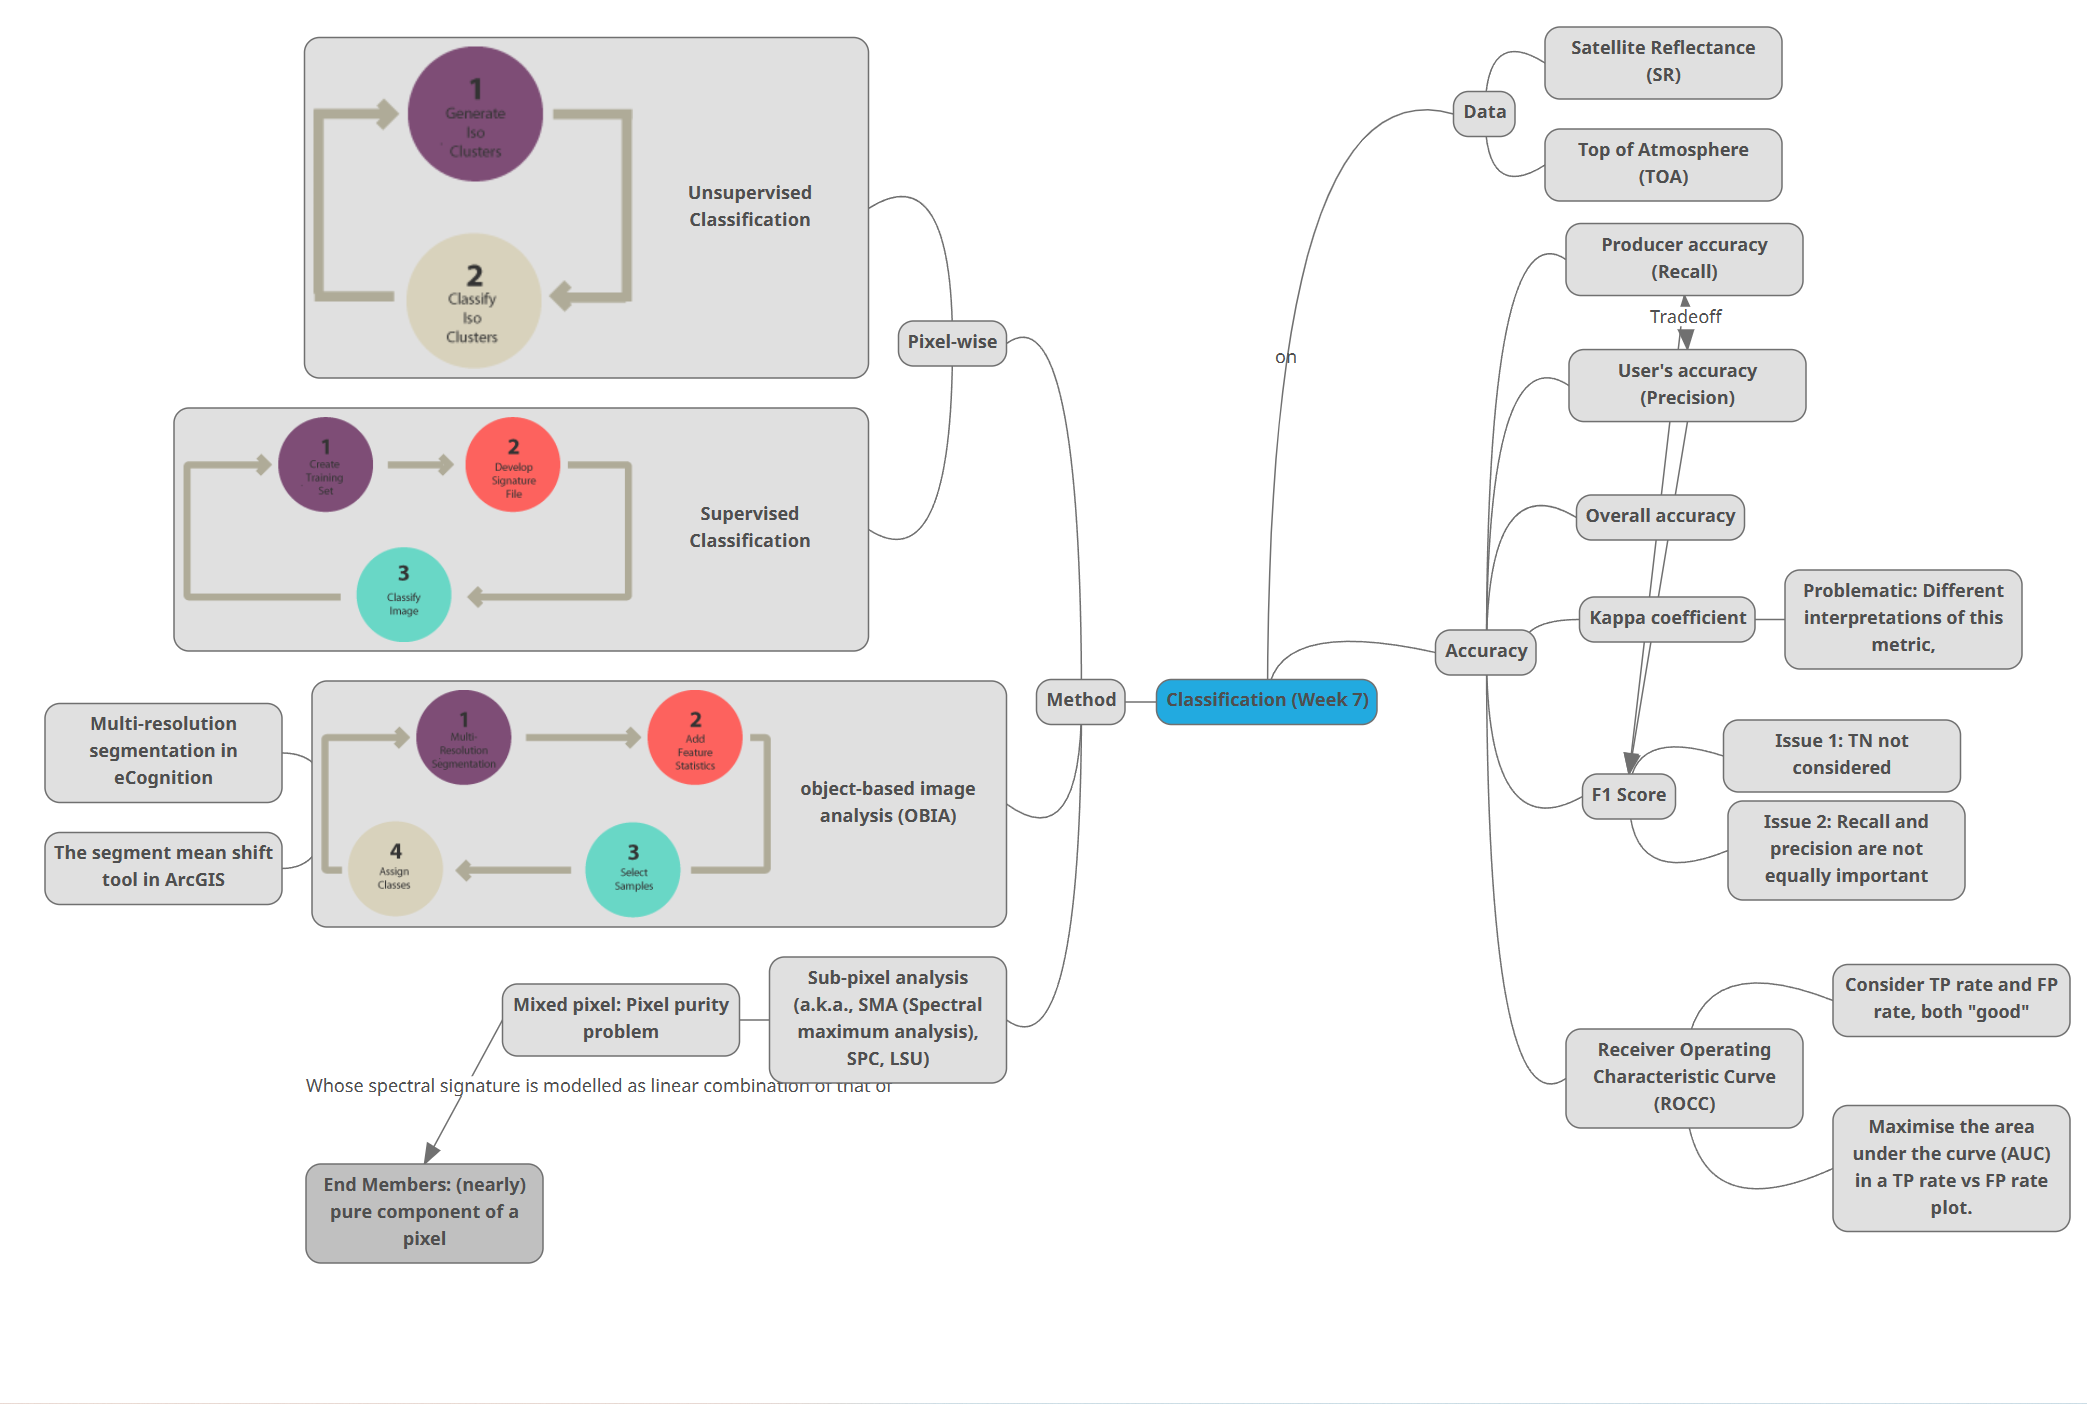
\includegraphics{./images/MindMap.png}

\hypertarget{data}{%
\subsection{Data}\label{data}}

\begin{itemize}
\item
  Surface Reflectance (SR)
\item
  Top of Atmosphere (TOA)
\end{itemize}

A mixed way of doing urban recognition

\hypertarget{obia-object-based-image-analysis}{%
\subsection{OBIA (object-based image
analysis)}\label{obia-object-based-image-analysis}}

Instead of a per-pixel approach, we adopt an object-based image analysis
(OBIA), where you have to manually create objects.

SLIC (\textbf{\emph{Simple~Linear~Iterative~Clustering}}) (2012): No
ground truth

Descent, similarity (Homogeneity)

\hypertarget{sub-pixel-analysis}{%
\subsection{Sub-pixel analysis}\label{sub-pixel-analysis}}

SMA (Spectral maximum analysis), SPC, LSU

Through a series of manipulation of material, we acquire a list
describing the broken-down land cover of that pixel

\hypertarget{pixel-purity}{%
\subsubsection{Pixel purity}\label{pixel-purity}}

\textbf{Endmember}: an important concept in spectral mixture analysis

In remote sensing, an end member refers to a pure or nearly pure
material or component that is present within a mixed pixel.

In spectral mixture analysis, the spectral signature of a mixed pixel is
modelled as a linear combination of the spectral signatures of the
constituent endmembers, with each end member being assigned a proportion
or fraction that represents its contribution to the overall reflectance
or radiance of the mixed pixel.

\hypertarget{accuracy-assessment}{%
\subsection{Accuracy assessment}\label{accuracy-assessment}}

\begin{itemize}
\item
  Producer accuracy: Recall
\item
  User's accuracy: Precision
\item
  Overall accuracy: not equivalent to F1
\item
  Kappa coefficient: {[}0, 1{]}, measures how good the classification is
  compared to random distribution e.g.~Poisson. Different
  interpretations of this metric, problematic
\end{itemize}

Make a tradeoff between Producer accuracy and User accuracy, by shifting
the decision boundary.

\begin{itemize}
\item
  F1: issue: TN not considered; Recall and precision are not equally
  important yet equally weighted in F1
\item
  Receiver Operating Characteristic Curve: True positive rate and false
  positive rate are all good. We want to maximise the area under the
  curve in a True positive rate vs false positive rate plot.
\end{itemize}

\hypertarget{workflow}{%
\subsection{Workflow}\label{workflow}}

\begin{itemize}
\item
  (Potentially use unsupervised classification to understand your data
\item
  Class definition (Potentially use unsupervised classification)
\item
  Preprocessing
\item
  Training
\item
  Pixel Assignment
\item
  Accuracy assessment
\end{itemize}

Pseudo-invariant features to be trained on to make your model robust to
time-space changes

Pseudo-invariant features are often used as reference targets or
calibration sites in remote sensing to account for changes in sensor or
atmospheric conditions and to reduce the effects of noise and
calibration drift on image data. These features have relatively constant
spectral properties over time and space, and can therefore serve as a
stable reference for monitoring changes in other features or materials
within an image or scene.

A flow chart can be seen in Figure~\ref{fig-flowchart} :

\begin{figure}

{\centering 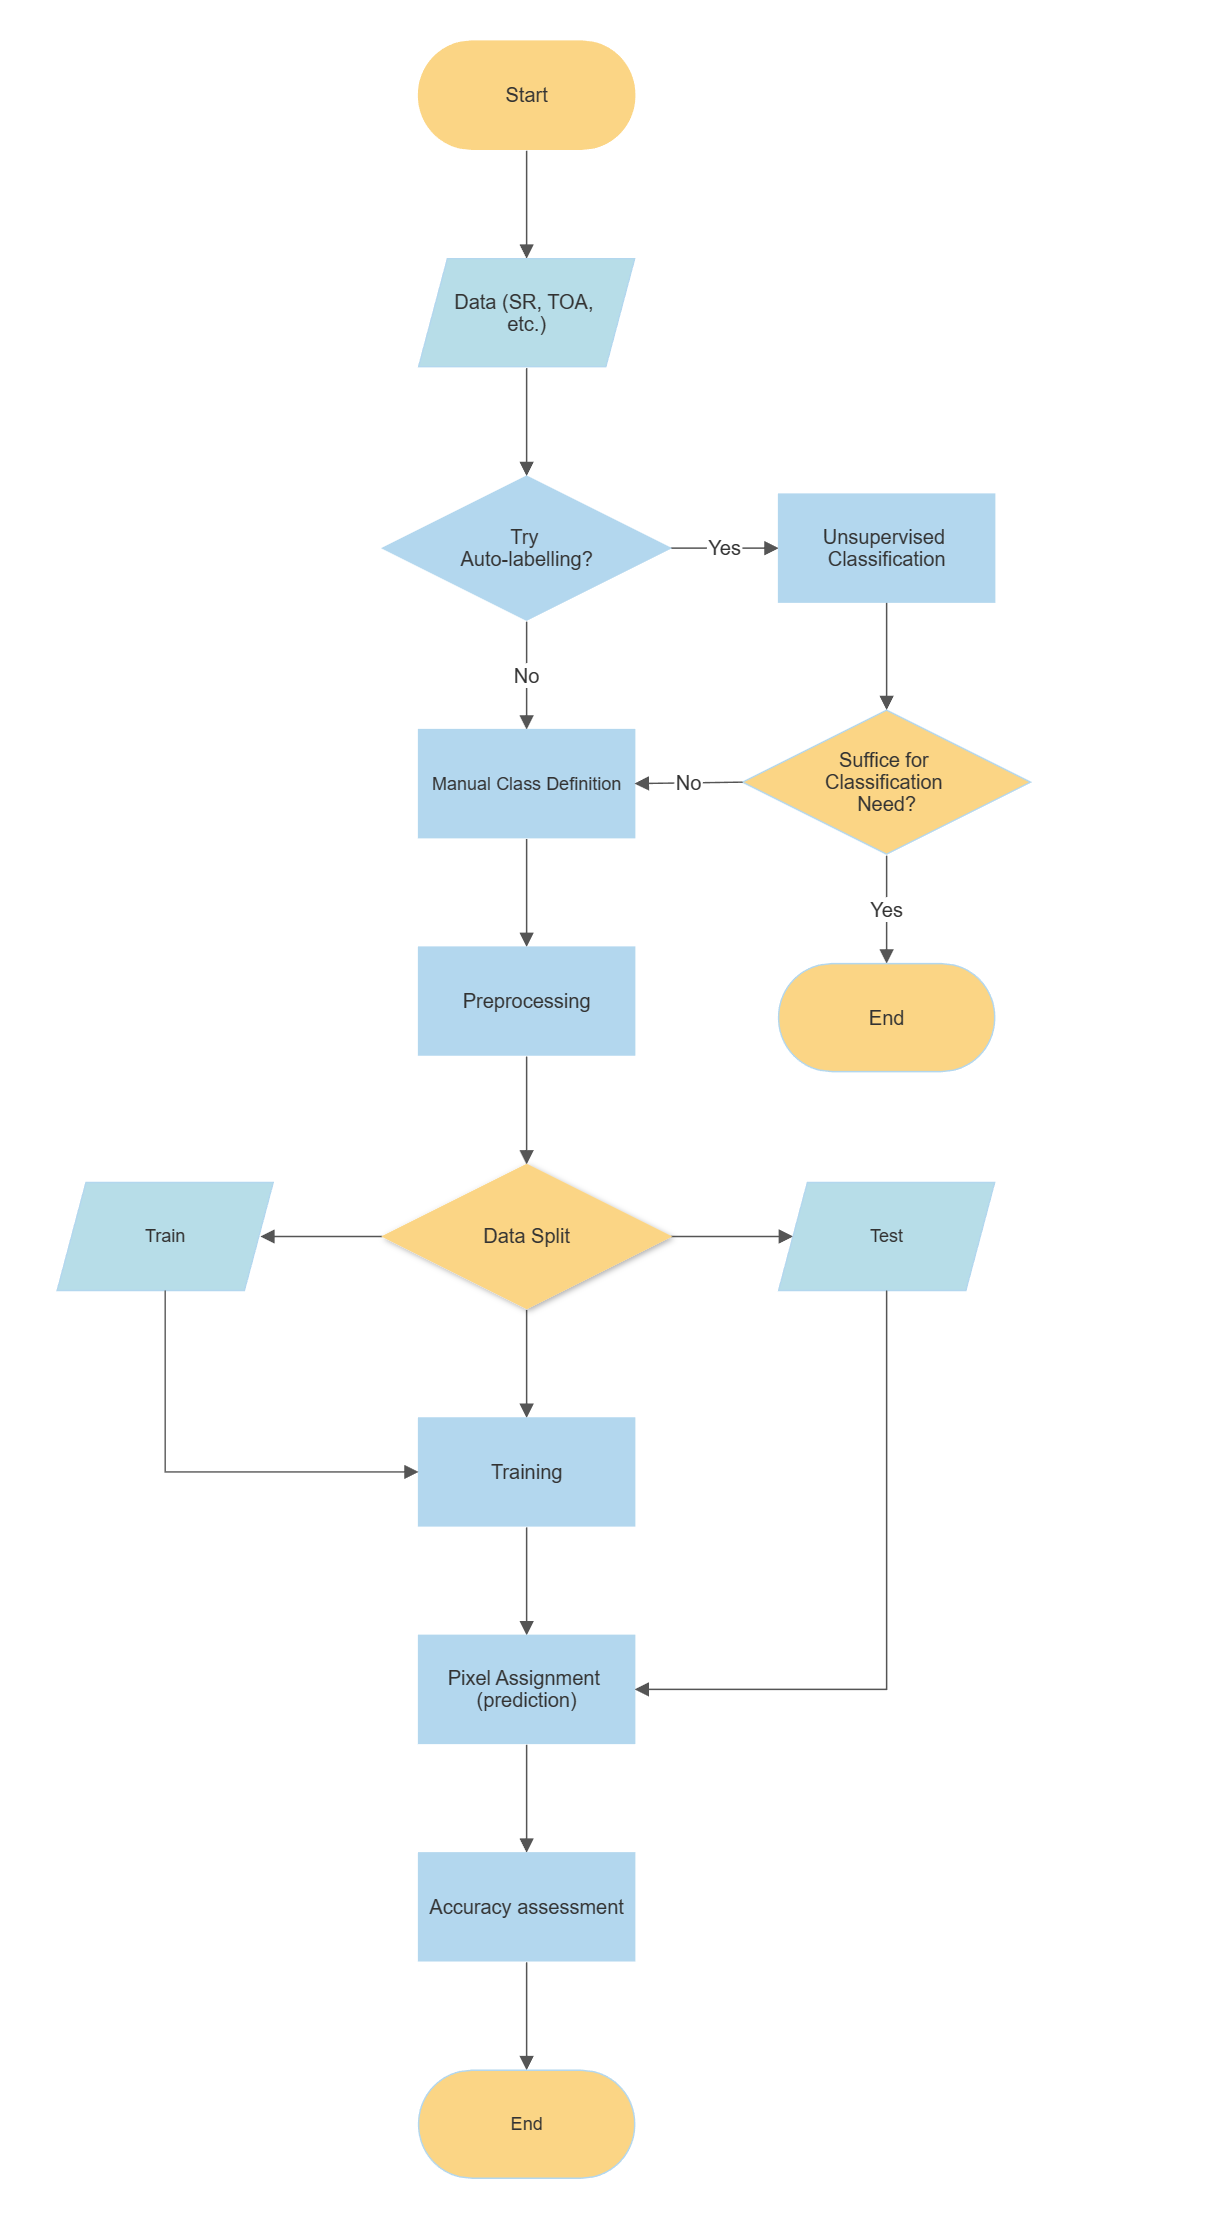
\includegraphics{./images/FlowChart.png}

}

\caption{\label{fig-flowchart}Classification Workflow, courtesy: myself}

\end{figure}

\hypertarget{a-sneak-preview-analogous-to-data-leakage-in-ml}{%
\subsection{A ``Sneak preview'' (Analogous to Data Leakage in
ML)}\label{a-sneak-preview-analogous-to-data-leakage-in-ml}}

Waldo Tobler's first law of geography indicates that if training and
testing are spatially close, the training can cause the problem of a
sneak preview.

\hypertarget{spatial-cross-validation}{%
\subsubsection{Spatial Cross
Validation}\label{spatial-cross-validation}}

Similar to cross-validation but adds clustering to folds.

In spatial cross-validation, the data are split into spatially
contiguous blocks or subsets, rather than randomly shuffled subsets as
in traditional cross-validation. This is done to ensure that the model
is tested on data that are spatially distinct from the data used to
train the model and to account for spatial autocorrelation and other
spatial dependencies in the data.

\hypertarget{approaches-to-deal-with-spatial-autocorrelation}{%
\subsection{Approaches to deal with Spatial
Autocorrelation}\label{approaches-to-deal-with-spatial-autocorrelation}}

Object-based image classification

Moran's I (Spatial Cross Validation)

\hypertarget{application---to-be-completed}{%
\section{Application - to be
completed}\label{application---to-be-completed}}

In remote sensing, it is often challenging to accurately classify mixed
pixels, which contain a combination of different materials or
components. Endmembers refer to pure or nearly pure materials that are
present within a mixed pixel. By modelling the spectral signature of a
mixed pixel as a linear combination of the spectral signatures of the
constituent endmembers, we can determine the contribution of each
endmember to the overall reflectance or radiance of the mixed pixel.

This approach can be very useful in urban recognition, where it is
essential to accurately classify the different land covers present
within a pixel. Furthermore, it can also help us to understand the
composition of the land cover in a given area, which can have important
implications for environmental monitoring and management. This approach
has been applied in various studies to estimate urban land cover, such
as the work by Zhang et al.~(2018) that utilised endmember extraction to
detect urban impervious surfaces.

\hypertarget{reflection-5}{%
\section{Reflection}\label{reflection-5}}

The workflow of Classification of Surface Reflectance and Top of
Atmosphere data intrigues me, as it differs from, yet shares certain
features with traditional computer vision tasks like image
classification and object detection (in regards of treating pixels as
objects/units). Alternatively, Surface Reflectance Classification can be
treated as a downstream task for both aforementioned ML tasks, due to
its uniqueness in dealing with high-precision satellite data and
unseparability (worth debating) from EO processing workflow (calibration
etc.). Also, uncertainty of classification genres derived from
unsupervised labelling can also be an issue.

Optionally, in supplementation to manual labelling, automated labelling
workflow (e.g.~roboflow) can be introduced to curtail repeatitive works
in image labelling(Nair, Paul, and Jacob 2018). However, manual
labelling is not replaceable at current time (Robison 2018) and the
pinning down of ground truth seems to always need human intervention in
addition to machine automation.

The introduction of production accuracy and user accuracy is also
interesting, as these terminologies are designed presupposing a
customer/producer split, dwarfing precision-recall in readability. The
treadeoff to be made between the two is crucial, and this is
problematically handled by introducing F1 score with two competitive
components, and improved by introducing Receiver Operating
Characteristic Curve (ROCC) with two ``good'' indicators, true positive
rate and false positive rate.

\bookmarksetup{startatroot}

\hypertarget{week8---temperature-and-policy}{%
\chapter{Week8 - Temperature and
Policy}\label{week8---temperature-and-policy}}

The ``policy'' section occupies two weeks, mainly trying to introduce
how to fit EO data workflow into current policies. To do this, you have
to identify the gaps, e.g., that between the overarching global
policies, metropolitan plans and local plans. Or, the gap within
policies like missing locations in the Singapore one.

\hypertarget{summary-6}{%
\section{Summary}\label{summary-6}}

\hypertarget{urban-heating-islands-uhi-problem-and-plans}{%
\subsection{Urban Heating Islands (UHI) problem and
plans}\label{urban-heating-islands-uhi-problem-and-plans}}

\hypertarget{causes}{%
\subsubsection{Causes}\label{causes}}

Urban areas have comparatively higher atmospheric and surface
temperatures than surrounding rural areas, mainly due to

\begin{enumerate}
\def\labelenumi{\arabic{enumi}.}
\tightlist
\item
  More dark surfaces that retain heat
\item
  Less vegetation that cools the environment
\end{enumerate}

Also, there are other contributors to the heat:

\begin{longtable}[]{@{}ll@{}}
\toprule()
Contributor & Correlation with UHI phenomenon \\
\midrule()
\endhead
Sky View Factor (SVF) & Positive \\
Air speed & Negative \\
Heavy cloud cover & Positive \\
Cyclic solar radiation & Positive \\
Building material type & Varies \\
Anthropogenic energy & Positive \\
\bottomrule()
\end{longtable}

\hypertarget{cost}{%
\subsubsection{Cost}\label{cost}}

The cost of the Urban Heat Island can be divided into social,
environmental, and economic costs.

\begin{longtable}[]{@{}
  >{\raggedright\arraybackslash}p{(\columnwidth - 2\tabcolsep) * \real{0.2535}}
  >{\raggedright\arraybackslash}p{(\columnwidth - 2\tabcolsep) * \real{0.7465}}@{}}
\toprule()
\begin{minipage}[b]{\linewidth}\raggedright
Type of Cost
\end{minipage} & \begin{minipage}[b]{\linewidth}\raggedright
Examples
\end{minipage} \\
\midrule()
\endhead
Social Costs & Population-adjusted excess mortality rates, heat-related
deaths \\
Environmental Costs & Increase in fossil fuel usage \\
Economic Costs & Loss of Gross Domestic Product (GDP) \\
\bottomrule()
\end{longtable}

For instance, under a low greenhouse gas scenario, the percent GDP lost
from UHI is estimated to be 0.71\% in 2050.

\hypertarget{plans}{%
\subsubsection{Plans}\label{plans}}

\hypertarget{global}{%
\paragraph{Global}\label{global}}

\hypertarget{local}{%
\paragraph{Local}\label{local}}

\begin{longtable}[]{@{}
  >{\raggedright\arraybackslash}p{(\columnwidth - 4\tabcolsep) * \real{0.2083}}
  >{\raggedright\arraybackslash}p{(\columnwidth - 4\tabcolsep) * \real{0.2917}}
  >{\raggedright\arraybackslash}p{(\columnwidth - 4\tabcolsep) * \real{0.5000}}@{}}
\toprule()
\begin{minipage}[b]{\linewidth}\raggedright
City
\end{minipage} & \begin{minipage}[b]{\linewidth}\raggedright
Initiatives
\end{minipage} & \begin{minipage}[b]{\linewidth}\raggedright
Technology
\end{minipage} \\
\midrule()
\endhead
Singapore & Green buildings & Urban greenery \\
Medellin & Green Corridors & Urban greenery \\
Sydney & Turn Down the Heat Strategy and Action Plan & Reflective
roofs/pavements/sidewalks, Cool roads trial in Western Sydney \\
\bottomrule()
\end{longtable}

\hypertarget{application-3}{%
\section{Application}\label{application-3}}

MacLachlan et al. (2021) The document outlines a sub-city urban planning
modeling approach using open-source tools to measure and monitor
localised urban heat island (UHI) mitigation targets. The methodology
involves comparing temperature dynamics of low- and high-density census
areas using Earth observation data and determining optimal placement of
greening elements in proposed plans using a data-driven model. The
document concludes that this approach can be universally integrated into
urban planning regulation frameworks to mitigate the localized UHI
effect and ensure long-term city sustainability. Also it discusses the
impact of low population density on housing in Perth, Australia, and the
resulting need for strategic land zonation and sustainability targets.
\#\#\#\# Why Data-driven approach

\hypertarget{policy-limitations}{%
\subsection{Policy limitations}\label{policy-limitations}}

\begin{itemize}
\tightlist
\item
  lacking \textbf{specificities} for combating adverse temperature
  effects at the local level (\textbf{sub-city}), therefore not planning
  practicality
\item
  no \textbf{consistency} in planning implementation
  \textbf{methodologies} or steps for \textbf{assessing} progress toward
  UHI reduction targets
\item
  lackage of empirical \textbf{evidence for optimizing} UHI mitigation
  strategies
\end{itemize}

\hypertarget{data-to-drive-the-new-approach}{%
\subsection{Data to drive the new
approach}\label{data-to-drive-the-new-approach}}

\begin{itemize}
\tightlist
\item
  Earth Observation (\textbf{EO}) data can be processed to identify
  (un)sustainable urban development through aerial assessments of
  \textbf{land cover change}
\item
  temperature
\item
  elevation
\end{itemize}

\hypertarget{advantages-for-the-data-driven-approach}{%
\subsection{Advantages for the Data-driven
approach}\label{advantages-for-the-data-driven-approach}}

\begin{itemize}
\tightlist
\item
  EO data can produce \textbf{consistent information} necessary for
  restricting unsustainable development
\item
  \textbf{monitor} UHI effects based on associated land-temperature
  dynamics
\item
  Assessment at finer spatial scales (e.g., block subdivisions)
\end{itemize}

\hypertarget{methodology}{%
\subsection{Methodology}\label{methodology}}

\begin{center}\rule{0.5\linewidth}{0.5pt}\end{center}

\hypertarget{temperature-modeling}{%
\subsubsection{Temperature Modeling}\label{temperature-modeling}}

\begin{center}\rule{0.5\linewidth}{0.5pt}\end{center}

\begin{itemize}
\tightlist
\item
  Modeled temperature every 3 hours using SOLWEIG model between 2008 and
  2010
\end{itemize}

\begin{center}\rule{0.5\linewidth}{0.5pt}\end{center}

\begin{itemize}
\tightlist
\item
  Inputs generated from meteorological data, land cover, building DSM,
  ground DTM, and vegetation canopy REM in QGIS
\end{itemize}

\begin{center}\rule{0.5\linewidth}{0.5pt}\end{center}

\begin{itemize}
\tightlist
\item
  SVF computed from vegetation canopy REM, building DSM, and ground DTM
  using UMEP plugin
\end{itemize}

\begin{center}\rule{0.5\linewidth}{0.5pt}\end{center}

\begin{itemize}
\tightlist
\item
  Building wall heights and aspect generated from DSM and DTM using UMEP
  plugin
\end{itemize}

\begin{center}\rule{0.5\linewidth}{0.5pt}\end{center}

\hypertarget{data-driven-tree-placement}{%
\subsubsection{Data-Driven Tree
Placement}\label{data-driven-tree-placement}}

\begin{center}\rule{0.5\linewidth}{0.5pt}\end{center}

\begin{itemize}
\tightlist
\item
  Site selected for modeling temperature in the City of Fremantle
\end{itemize}

\begin{center}\rule{0.5\linewidth}{0.5pt}\end{center}

\begin{itemize}
\tightlist
\item
  Three scenarios processed: current urban footprint, proposed changes,
  and proposed redevelopment with no trees
\end{itemize}

\begin{center}\rule{0.5\linewidth}{0.5pt}\end{center}

\begin{itemize}
\tightlist
\item
  Highest temperatures identified and used to redesign tree placement
\end{itemize}

\begin{center}\rule{0.5\linewidth}{0.5pt}\end{center}

\begin{itemize}
\tightlist
\item
  15 trees distributed according to original design aspects
\end{itemize}

\begin{center}\rule{0.5\linewidth}{0.5pt}\end{center}

\begin{itemize}
\tightlist
\item
  Updated vegetation canopy REM reflected new tree locations
\end{itemize}

\begin{center}\rule{0.5\linewidth}{0.5pt}\end{center}

\begin{itemize}
\tightlist
\item
  Analysis re-run to compare temperature across redevelopment site
\end{itemize}

\begin{center}\rule{0.5\linewidth}{0.5pt}\end{center}

\begin{itemize}
\tightlist
\item
  Modeled all scenarios accounting for influence of neighboring
  landscape features
\end{itemize}

\begin{center}\rule{0.5\linewidth}{0.5pt}\end{center}

\hypertarget{result}{%
\subsection{Result}\label{result}}

Table 1: Results of assessments of urban design factors on UHI effect in
Perth.

\begin{longtable}[]{@{}ll@{}}
\toprule()
Factors assessed & Effect on UHI effect \\
\midrule()
\endhead
Vegetation cover & Negative correlation with UHI effect \\
Canopy cover & Negative correlation with UHI effect \\
Building density & Positive correlation with UHI effect \\
Building height & Positive correlation with UHI effect \\
Albedo & Negative correlation with UHI effect \\
Land use & Negative correlation with UHI effect \\
Urban sprawl & Positive correlation with UHI effect \\
\bottomrule()
\end{longtable}

Table 2: Total population and population density per 0.1 km2 between
2011 and 2016 for Subiaco and Currambine SA1s as defined by the ABS.

\begin{longtable}[]{@{}
  >{\raggedright\arraybackslash}p{(\columnwidth - 8\tabcolsep) * \real{0.1892}}
  >{\raggedright\arraybackslash}p{(\columnwidth - 8\tabcolsep) * \real{0.1892}}
  >{\raggedright\arraybackslash}p{(\columnwidth - 8\tabcolsep) * \real{0.1892}}
  >{\raggedright\arraybackslash}p{(\columnwidth - 8\tabcolsep) * \real{0.2162}}
  >{\raggedright\arraybackslash}p{(\columnwidth - 8\tabcolsep) * \real{0.2162}}@{}}
\toprule()
\begin{minipage}[b]{\linewidth}\raggedright
\textbf{SA1}
\end{minipage} & \begin{minipage}[b]{\linewidth}\raggedright
\textbf{Total Population (2011)}
\end{minipage} & \begin{minipage}[b]{\linewidth}\raggedright
\textbf{Total Population (2016)}
\end{minipage} & \begin{minipage}[b]{\linewidth}\raggedright
\textbf{Population Density per 0.1 km2 (2011)}
\end{minipage} & \begin{minipage}[b]{\linewidth}\raggedright
\textbf{Population Density per 0.1 km2 (2016)}
\end{minipage} \\
\midrule()
\endhead
Subiaco & N/A & N/A & 325 & 712 \\
Currambine & N/A & N/A & 310 & 324 \\
\bottomrule()
\end{longtable}

\hypertarget{reflection-6}{%
\section{Reflection}\label{reflection-6}}

\begin{itemize}
\tightlist
\item
  Case study: Superblocks, Barcelona
\end{itemize}

Basically about pedestrian economy. Though there have been many retail
modes like KFC and other American fast food, the experience from Europe
tells that economy vitality can have a boost with pedestrian-dominated
areas. See Barcelona

\bookmarksetup{startatroot}

\hypertarget{week-9---synthetic-aperture-radar-sar-data}{%
\chapter{Week 9 - Synthetic Aperture Radar (SAR)
data}\label{week-9---synthetic-aperture-radar-sar-data}}

\hypertarget{summary-7}{%
\section{Summary}\label{summary-7}}

\hypertarget{a-quick-overview}{%
\subsection{A quick overview}\label{a-quick-overview}}

This week addresses problems in

\begin{itemize}
\tightlist
\item
  The object of using Synthetic Aperture Radar (SAR)
\end{itemize}

Detecting changes in the Earth's surface over time

\begin{itemize}
\item
  The advantages of SAR for change detection

  \begin{itemize}
  \tightlist
  \item
    see through clouds
  \item
    high temporal resolution
  \end{itemize}
\item
  Techniques for change detection with SAR?

  \begin{itemize}
  \tightlist
  \item
    ratio
  \item
    log ratios between two images
  \item
    t-tests
  \end{itemize}
\item
  fused with other data?

  Yes, with optical data using techniques such as

  \begin{enumerate}
  \def\labelenumi{\arabic{enumi}.}
  \tightlist
  \item
    principal component analysis
  \item
    object-based image analysis
  \item
    intensity fusion
  \end{enumerate}
\item
  Applications?

  \begin{itemize}
  \tightlist
  \item
    monitoring land use changes
  \item
    detecting deforestation
  \item
    identifying urban growth pattern
  \end{itemize}
\end{itemize}

\hypertarget{sar-fundamentals}{%
\subsection{SAR fundamentals}\label{sar-fundamentals}}

\begin{itemize}
\item
  Definition: Synthetic Aperture Radar (SAR) is a type of radar that
  uses microwave signals to create high-resolution images of the Earth's
  surface.
\item
  Advantages:

  \begin{itemize}
  \tightlist
  \item
    Operates in all weather conditions
  \item
    Penetrates through clouds and vegetation cover.
  \end{itemize}
\item
  Limitations

  \begin{itemize}
  \tightlist
  \item
    Sensitive to surface roughness; limited spatial resolution.
  \end{itemize}
\item
  Processing Techniques

  \begin{itemize}
  \tightlist
  \item
    Interferometry: combines multiple SAR images to create 3D maps of
    the Earth's surface.
  \item
    Polarimetry: analyzes the polarization properties of reflected
    signals to extract additional information about surface features.
  \end{itemize}

  The relationship between different surfaces and their sensitivity to
  polarizations in SAR data

  \begin{longtable}[]{@{}
    >{\raggedright\arraybackslash}p{(\columnwidth - 4\tabcolsep) * \real{0.2083}}
    >{\raggedright\arraybackslash}p{(\columnwidth - 4\tabcolsep) * \real{0.2292}}
    >{\raggedright\arraybackslash}p{(\columnwidth - 4\tabcolsep) * \real{0.5625}}@{}}
  \toprule()
  \begin{minipage}[b]{\linewidth}\raggedright
  Surface Type
  \end{minipage} & \begin{minipage}[b]{\linewidth}\raggedright
  Scattering Mechanism
  \end{minipage} & \begin{minipage}[b]{\linewidth}\raggedright
  Most Sensitive Polarization
  \end{minipage} \\
  \midrule()
  \endhead
  Rough (bare earth) & Rough Scattering & Vertical-Vertical (VV) \\
  Leaves & Volume Scattering & Vertical-Horizontal (VH) or
  Horizontal-Vertical (HV) \\
  Trees / Buildings & Double Bounce & Horizontal-Horizontal (HH) \\
  \bottomrule()
  \end{longtable}
\item
  Applications:

  \begin{itemize}
  \tightlist
  \item
    Environmental monitoring, disaster response, urban planning,
    military surveillance, and more.
  \end{itemize}
\end{itemize}

\hypertarget{practical-change-detection-with-sar}{%
\subsection{Practical change detection with
SAR}\label{practical-change-detection-with-sar}}

\begin{longtable}[]{@{}
  >{\raggedright\arraybackslash}p{(\columnwidth - 2\tabcolsep) * \real{0.3007}}
  >{\raggedright\arraybackslash}p{(\columnwidth - 2\tabcolsep) * \real{0.6993}}@{}}
\toprule()
\begin{minipage}[b]{\linewidth}\raggedright
Topic
\end{minipage} & \begin{minipage}[b]{\linewidth}\raggedright
Key Points
\end{minipage} \\
\midrule()
\endhead
Advantages of SAR for Change Detection & Can see through clouds unlike
optical sensors; high temporal resolution. \\
Change Detection Techniques & Ratio or log ratios between two images;
t-tests; standard deviation. \\
Fusion of SAR and Optical Data & Principal component analysis;
object-based image analysis; intensity fusion. \\
Applications of Change Detection with SAR & Monitoring land use changes,
detecting deforestation, identifying urban growth patterns, and more. \\
\bottomrule()
\end{longtable}

\hypertarget{possible-future-developments}{%
\subsection{Possible future
developments}\label{possible-future-developments}}

Resolution, accuracy, real-time-ness and data scale in SAR might see
advancements.

\begin{itemize}
\item
  Improved resolution and accuracy:

  \begin{itemize}
  \tightlist
  \item
    Urban planning: Improved resolution and accuracy can influence local
    zoning regulations and urban growth management by providing detailed
    information on land use changes and the built environment. For
    example, high-resolution SAR data can be used to assess the
    effectiveness of urban containment policies or to identify areas
    where infrastructure investments are needed.
  \end{itemize}
\item
  Data processing capabilities

  \begin{itemize}
  \tightlist
  \item
    Disaster response: The ability to process larger datasets and
    monitor Earth's surface in near real-time can inform global policies
    regarding disaster management, such as the
    \href{https://www.undrr.org/implementing-sendai-framework/what-sendai-framework}{Sendai
    Framework for Disaster Risk Reduction}. Boosted rapidness and data
    capability of SAR can better response to natural disasters, like
    earthquakes or hurricanes. This allows for quicker design of
    resources deployment strategy, and more comprehensive information in
    managing affected areas.
  \end{itemize}
\item
  New SAR applications

  \begin{itemize}
  \tightlist
  \item
    Agricultural: Enhanced SAR facilitates its use in change detection
    and monitoring. This will support policies like the
    \href{https://ec.europa.eu/info/food-farming-fisheries/key-policies/common-agricultural-policy/cap-glance_en}{European
    Union's Common Agricultural Policy (CAP)}, by providing data on crop
    health, irrigation needs, and land use changes.
  \item
    Forestry (deforestation and reforestation tracking)
  \item
    Disaster response (flood and landslide monitoring)
  \item
    Environmental management: SAR data can inform policies related to
    wetland and coastal zone management, such as the
    \href{https://www.ramsar.org/}{Ramsar Convention on Wetlands} and
    the
    \href{https://www.un.org/Depts/los/convention_agreements/convention_overview_convention.htm}{United
    Nations Convention on the Law of the Sea (UNCLOS)}. By monitoring
    changes in these sensitive areas, policymakers can evaluate the
    effectiveness of existing regulations and develop new strategies to
    protect vital ecosystems.
  \end{itemize}
\item
  More matured machine learning and artificial intelligence:

  \begin{itemize}
  \tightlist
  \item
    Advanced algorithms that are yet to be developed or need further
    maturity for SAR data analysis could include:
  \end{itemize}

  \begin{longtable}[]{@{}
    >{\raggedright\arraybackslash}p{(\columnwidth - 4\tabcolsep) * \real{0.1409}}
    >{\raggedright\arraybackslash}p{(\columnwidth - 4\tabcolsep) * \real{0.4807}}
    >{\raggedright\arraybackslash}p{(\columnwidth - 4\tabcolsep) * \real{0.3785}}@{}}
  \toprule()
  \begin{minipage}[b]{\linewidth}\raggedright
  Algorithm
  \end{minipage} & \begin{minipage}[b]{\linewidth}\raggedright
  Pros
  \end{minipage} & \begin{minipage}[b]{\linewidth}\raggedright
  Cons
  \end{minipage} \\
  \midrule()
  \endhead
  Improved Unsupervised Change Detection Algorithms & - No need for
  labeled training data. - Can discover unknown or unexpected changes. &
  - May struggle with complex or subtle changes. - Can be sensitive to
  noise and variations in the data. \\
  Multi-Modal Fusion Algorithms & - Combines SAR data with other sources
  (e.g., optical, hyperspectral) for better feature identification. -
  Can exploit the complementary strengths of different data types. & -
  Requires data synchronization and registration, which can be
  challenging. - May involve increased complexity and computational
  cost. \\
  Graph-based Change Detection Algorithms & - Can model complex spatial
  relationships between features. - Robust against noise and speckle
  effects in SAR data. & - Computationally expensive, especially for
  large-scale datasets. - May require tuning of hyperparameters. \\
  \bottomrule()
  \end{longtable}

  \begin{itemize}
  \tightlist
  \item
    Improved overall accuracy of change detection can support climate
    change adaptation efforts at both local and global levels, including
    the \href{https://unfccc.int/}{United Nations Framework Convention
    on Climate Change (UNFCCC)} and the \href{https://unfccc.int/}{Paris
    Agreement}. Predictive models based on SAR data can help
    policymakers identify areas at risk of flooding, coastal erosion, or
    other climate-related impacts, enabling the targeted adaptation
    strategies.
  \end{itemize}
\end{itemize}

Advancements in SAR technology, combined with the integration of machine
learning and AI, will enhance change detection capabilities, enabling
new analysis avenues in sectors including agriculture, forestry,
disaster management, and environmental protection, ultimately
influencing policymaking and promoting more informed decision-making
processes.

\hypertarget{application-4}{%
\section{Application}\label{application-4}}

This week I chose to explore the application of SAR in wetland
classification and real-time monitoring, as well as its future
advancement, in the context of a literature recommended by the module
webpage (Dabboor and Brisco 2019).

Wetland acts as a kidney to Earth reminding one of the old positivist
tradition in French philosophy, taking abstract structures as organisms.
The chance to explore this wholist view with an analytic approach is
thrilling, as these two paradigms that seem to be falling in a
prevailing antithesis can actually sparkle inspiration and exhibit
harmony of inclusion of each other.

\hypertarget{wetland-classification}{%
\subsection{Wetland classification}\label{wetland-classification}}

Wetland classification has been a daunting task utilising traditional
air photo and filed visits. Ever since the launch of ERTS in 1972, this
task has been expecting the evolution of methods through applying Earth
Observation data.

The SOTA of this tasks, as implied in the literature, has been an
Object-based classification:

\begin{itemize}
\tightlist
\item
  Combining multi-source data: optical and SAR
\item
  Analysing using a machine-learning classification model
\item
  Incorporating a Digital Elevation Model (DEM)
\item
  Aims at identifying terrain suitability for wetlands and surface water
\end{itemize}

See @ for a workflow

This method achieves over 90\% of accuracy and is useful in that its
core method utilises SAR data's feature of ``seeing under the water'' to
better identify flooded vegetation class.

How did this amazing feature come about? Is that an emerging effect due
to unprecedented combination of data? Or is it determined by the
characteristics innate to SAR data?

The answer is the latter: The flooded vegetation tends to produce a
double bounce scattering mechanism, which increases the intensity of the
backscatter, making HH polarization to be the best for this due to the
enhanced penetration in vegetation (\textbf{Jahncke2018MappingWI?}).

\begin{figure}

{\centering 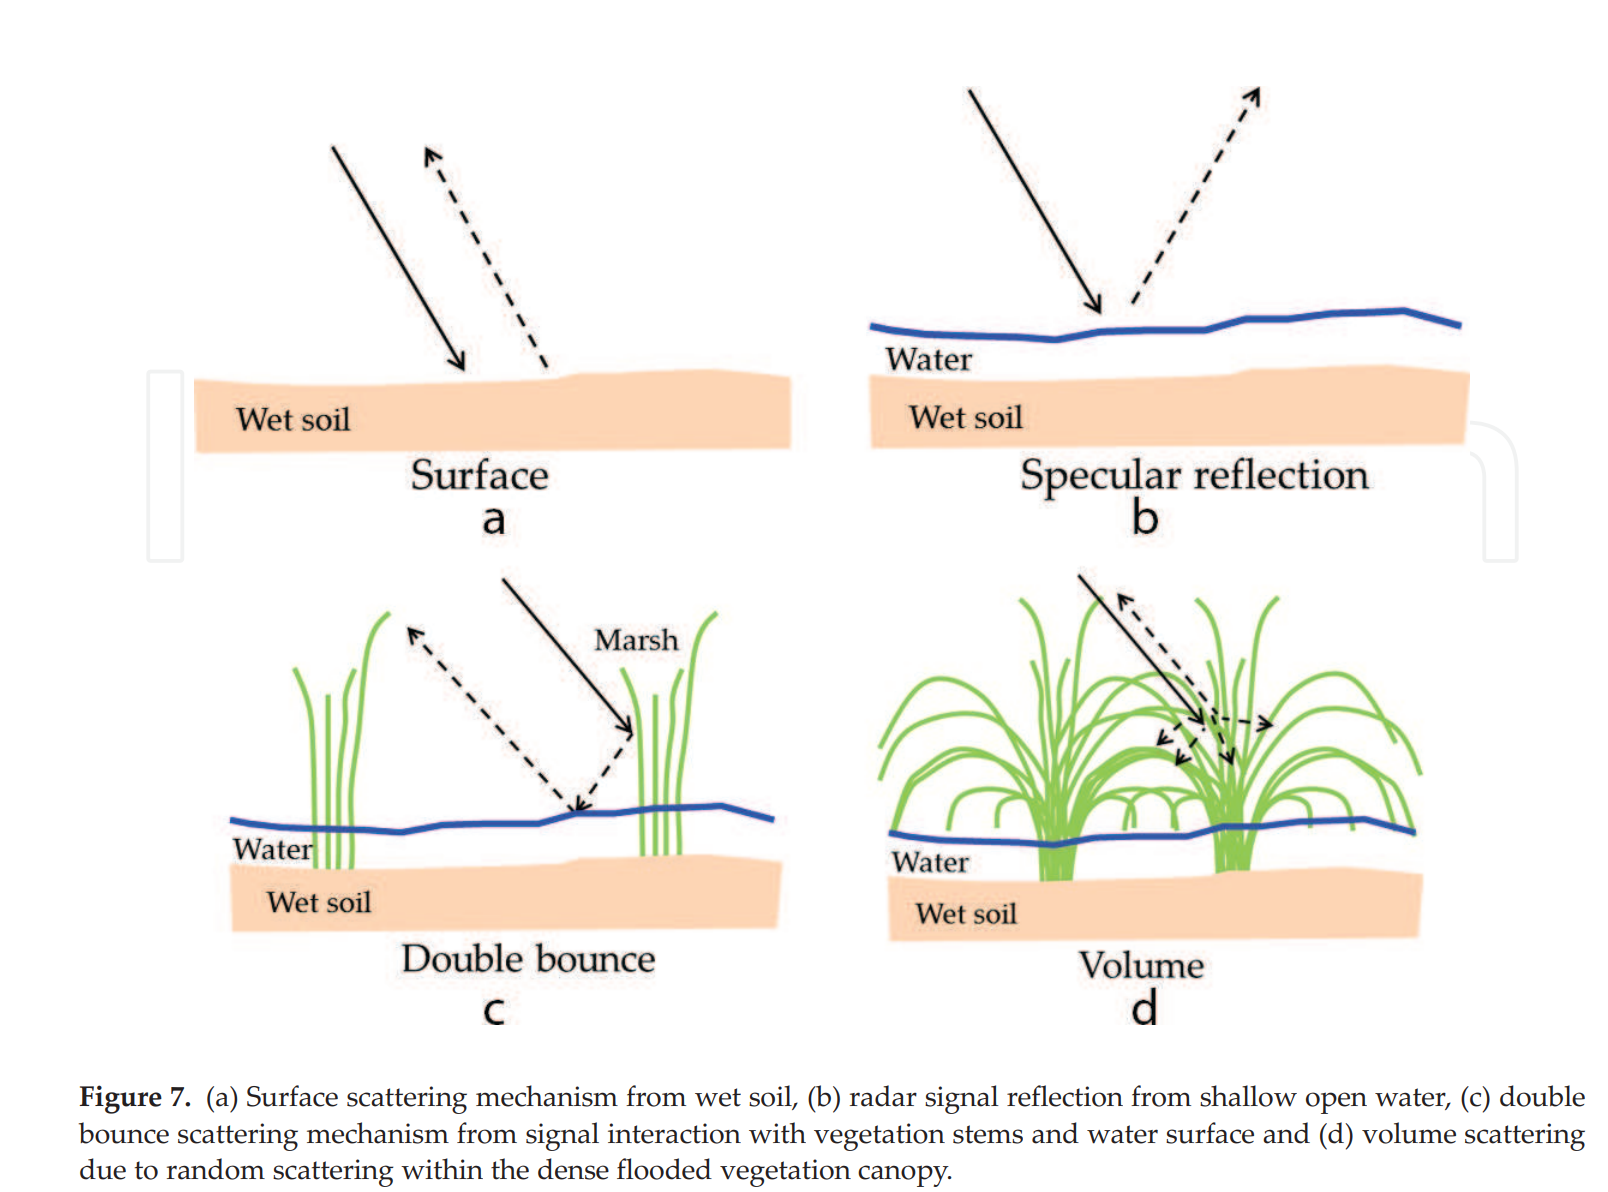
\includegraphics{./images/WetLand_classification.png}

}

\caption{Credit: Dabboor and Brisco (2019)}

\end{figure}

This workflow utilising different scattering effect between water and
vegetation is one of the main contributors to the SOTA performance,
laying the ground for further development and iteration on this method:
various angle-choosing strategies, machine-learning algorithm
combinations, etc.

\hypertarget{future-advancement-1}{%
\subsection{Future Advancement}\label{future-advancement-1}}

\begin{itemize}
\tightlist
\item
  Resolution in time and space can see chance of enhancement. Spaceborne
  SAR remote sensing technology being the essential tool for effective
  wetland observation, its improvement can be expected to reflect on
  enhancement of wetland observation in temporal and spatial resolution,
  e.g., the RCM is expected to provide SAR imagery in a spatial
  resolution ranging from 1 m to 100 m, in a revisit time of only 4 days
  (Dabboor and Brisco 2019).
\end{itemize}

This can better our understanding of climate change in wetlands and
water quality, allowing ecosystem managers and decision makers to have
sufficient information regarding wetland preservation

\begin{itemize}
\tightlist
\item
  More sensors with more data forms, as well as improved data quality
  can be anticipated in the future. The integration of SAR imagery with
  optical and topographic data from multiple sensors was shown in Dubeau
  et al. (2017) to be necessary for improved wetland mapping and
  classification during the growing season.
\end{itemize}

However, the integration of SAR imagery and LiDAR data did not improve
significantly the classification accuracy of wetland in Millard and
Richardson (2013).

\begin{itemize}
\tightlist
\item
  The effectiveness of machine learning algorithms for automated wetland
  classification can expect further development. E.g., Graph-based
  Change Detection Algorithms can model complex spatial relationships
  between features and is robust against noise and speckle effects in
  SAR data.
\end{itemize}

This shift toward the automated machine learning algorithms comes to
fulfill the requirement for operational wetland monitoring systems.

\bookmarksetup{startatroot}

\hypertarget{summary-8}{%
\chapter{Summary}\label{summary-8}}

In summary, this book has no content whatsoever.

\begin{Shaded}
\begin{Highlighting}[]
\DecValTok{1} \OperatorTok{+} \DecValTok{1}
\end{Highlighting}
\end{Shaded}

\begin{verbatim}
2
\end{verbatim}

\bookmarksetup{startatroot}

\hypertarget{references}{%
\chapter*{References}\label{references}}
\addcontentsline{toc}{chapter}{References}

\hypertarget{refs}{}
\begin{CSLReferences}{1}{0}
\leavevmode\vadjust pre{\hypertarget{ref-butcher_tour_2016}{}}%
Butcher, Ginger. 2016. \emph{Tour of the Electromagnetic Spectrum}.
Third edition. Washington, DC: National Aeronautics; Space
Administration.

\leavevmode\vadjust pre{\hypertarget{ref-gokce_wetland_2019}{}}%
Dabboor, Mohammed, and Brian Brisco. 2019. {``Wetland {Monitoring} and
{Mapping} {Using} {Synthetic} {Aperture} {Radar}.''} In \emph{Wetlands
{Management} - {Assessing} {Risk} and {Sustainable} {Solutions}}, edited
by Didem Gökçe. IntechOpen.
\url{https://doi.org/10.5772/intechopen.80224}.

\leavevmode\vadjust pre{\hypertarget{ref-dubeau_mapping_2017}{}}%
Dubeau, Pierre, Douglas J. King, Dikaso Gojamme Unbushe, and Lisa-Maria
Rebelo. 2017. {``Mapping the {Dabus} {Wetlands}, {Ethiopia}, {Using}
{Random} {Forest} {Classification} of {Landsat}, {PALSAR} and
{Topographic} {Data}.''} \emph{Remote Sensing} 9 (10).
\url{https://doi.org/10.3390/rs9101056}.

\leavevmode\vadjust pre{\hypertarget{ref-google_machine_2023}{}}%
Google. 2023a. {``Machine {Learning} in {Earth} {Engine} {\textbar}
{Google} {Earth} {Engine}.''} \emph{Google Developers}.
\url{https://developers.google.com/earth-engine/guides/machine-learning}.

\leavevmode\vadjust pre{\hypertarget{ref-google_reducer_2023}{}}%
---------. 2023b. {``Reducer {Overview} {\textbar} {Google} {Earth}
{Engine}.''} \emph{Google Developers}.
\url{https://developers.google.com/earth-engine/guides/reducers_intro}.

\leavevmode\vadjust pre{\hypertarget{ref-gorelick_google_2017}{}}%
Gorelick, Noel, Matt Hancher, Mike Dixon, Simon Ilyushchenko, David
Thau, and Rebecca Moore. 2017. {``Google {Earth} {Engine}:
{Planetary}-Scale Geospatial Analysis for Everyone.''} \emph{Remote
Sensing of Environment}, Big {Remotely} {Sensed} {Data}: Tools,
applications and experiences, 202 (December): 18--27.
\url{https://doi.org/10.1016/j.rse.2017.06.031}.

\leavevmode\vadjust pre{\hypertarget{ref-Jensen1986IntroductoryDI}{}}%
Jensen, J. Robert. 1986. {``Introductory Digital Image Processing: A
Remote Sensing Perspective.''} In.

\leavevmode\vadjust pre{\hypertarget{ref-maclachlan_sustainable_2021}{}}%
MacLachlan, Andrew, Eloise Biggs, Gareth Roberts, and Bryan Boruff.
2021. {``Sustainable {City} {Planning}: {A} {Data}-{Driven} {Approach}
for {Mitigating} {Urban} {Heat}.''} \emph{Frontiers in Built
Environment} 6.
\url{https://www.frontiersin.org/articles/10.3389/fbuil.2020.519599}.

\leavevmode\vadjust pre{\hypertarget{ref-millard_wetland_2013}{}}%
Millard, Koreen, and Murray Richardson. 2013. {``Wetland Mapping with
{LiDAR} Derivatives, {SAR} Polarimetric Decompositions, and
{LiDAR}--{SAR} Fusion Using a Random Forest Classifier.''}
\emph{Canadian Journal of Remote Sensing} 39 (4): 290--307.
\url{https://doi.org/10.5589/m13-038}.

\leavevmode\vadjust pre{\hypertarget{ref-moore_google_2011}{}}%
Moore, R., and M. Hansen. 2011. {``Google {Earth} {Engine}: A New
Cloud-Computing Platform for Global-Scale Earth Observation Data and
Analysis.''} \emph{AGU Fall Meeting Abstracts}, December, 02.

\leavevmode\vadjust pre{\hypertarget{ref-nair2018automated}{}}%
Nair, Rahul, P. J. Paul, and K. Poulose Jacob. 2018. {``Automated Image
Annotation: A Survey.''} \emph{Journal of Imaging} 4 (3): 37.

\leavevmode\vadjust pre{\hypertarget{ref-robison2018future}{}}%
Robison, Keela. 2018. {``The Future of Image Annotation: Human in the
Loop.''}
\url{https://lionbridge.ai/articles/the-future-of-image-annotation-human-in-the-loop/}.

\leavevmode\vadjust pre{\hypertarget{ref-saad_el_imanni_multispectral_2023}{}}%
Saad El Imanni, Hajar, Abderrazak El Harti, El Mostafa Bachaoui, Hicham
Mouncif, Fatine Eddassouqui, Mohamed Achraf Hasnai, and Moulay Ismail
Zinelabidine. 2023. {``Multispectral {UAV} Data for Detection of Weeds
in a Citrus Farm Using Machine Learning and {Google} {Earth} {Engine}:
{Case} Study of {Morocco}.''} \emph{Remote Sensing Applications: Society
and Environment} 30 (April): 100941.
\url{https://doi.org/10.1016/j.rsase.2023.100941}.

\leavevmode\vadjust pre{\hypertarget{ref-schulte_to_buhne_better_2018}{}}%
Schulte to Bühne, Henrike, and Nathalie Pettorelli. 2018. {``Better
Together: {Integrating} and Fusing Multispectral and Radar Satellite
Imagery to Inform Biodiversity Monitoring, Ecological Research and
Conservation Science.''} \emph{Methods in Ecology and Evolution} 9 (4):
849--65. \url{https://doi.org/10.1111/2041-210X.12942}.

\end{CSLReferences}



\end{document}
